% %%%%%%%% ICML 2019 EXAMPLE LATEX SUBMISSION FILE %%%%%%%%%%%%%%%%%
%\documentclass{article}
%% Recommended, but optional, packages for figures and better typesetting:
%\usepackage{microtype}
%\usepackage{graphicx}
%%\usepackage{subfigure}
%\usepackage{booktabs} % for professional tables
%% hyperref makes hyperlinks in the resulting PDF.
%% If your build breaks (sometimes temporarily if a hyperlink spans a page)
%% please comment out the following usepackage line and replace
%% \usepackage{icml2019} with \usepackage[nohyperref]{icml2019} above.
%\usepackage{hyperref}
%% Attempt to make hyperref and algorithmic work together better:
%%\newcommand{\theHalgorithm}{\arabic{algorithm}}
%% If accepted, instead use the following line for the camera-ready submission:
%\usepackage[accepted]{icml2019}
%
%%%% BEGIN our stuff
%\RequirePackage[table]{xcolor}
%\usepackage{multirow}
%\usepackage{makecell}
%\usepackage{pifont}% http://ctan.org/pkg/pifont
%\newcommand{\cmark}{\ding{51}}%
%\newcommand{\xmark}{\ding{55}}%
%\usepackage{amsmath,amssymb}
%\usepackage{dsfont}
%% \usepackage{bbm}
%\usepackage{caption,subcaption}
%\usepackage[noend]{algpseudocode}  % Note: Had to disable algorithmic in icml2019.sty
%\usepackage[12pt]{moresize}
%
%\newcommand{\fix}{\marginpar{FIX}}
%\newcommand{\new}{\marginpar{NEW}}
%%%% END our stuff
\chapter{How to Learn Network Architecture like a Decision Tree}
\label{chapter:ant}

\paragraph{Abstract:} Deep neural networks and decision trees operate on largely separate paradigms; typically, the former performs representation learning with pre-specified architectures, while the latter is characterised by learning hierarchies over pre-specified features with learned architectures. We unite the two via \emph{adaptive neural trees} (ANTs) that incorporates representation learning into edges, routing functions and leaf nodes of a decision tree, along with a backpropagation-based training algorithm that adaptively grows the architecture from primitive modules (e.g., convolutional layers). We demonstrate that, whilst achieving competitive performance on classification and regression datasets, ANTs benefit from (i) lightweight inference via conditional computation, (ii) hierarchical separation of features useful to the task e.g. learning meaningful class associations, such as separating natural vs. man-made objects, and (iii) a mechanism to adapt the architecture to the size and complexity of the training dataset. This chapter is based on \cite{AdaptiveNeuralTrees19}. 

%
\section{Introduction}
Neural networks (NNs) and decision trees (DTs) are both powerful classes of machine learning models with proven successes in academic and commercial applications. The two approaches, however, typically come with mutually exclusive benefits and limitations.

%DNNs are characterised by learning hierarchical representation of data \cite{zeiler2014visualizing,bengio2013deep}. In the supervised learning setting, DNNs are capable of learning complex non-linear transformations to apply to input data, so a simple linear model can adequately perform the predictive task of interest.
NNs are characterised by learning hierarchical representations of data through the composition of nonlinear transformations \cite{zeiler2014visualizing,bengio2013deep}, % In classification, for example, the final representations of different classes are trained to become linearly separable.
which has alleviated the need for feature engineering, in contrast with many other machine learning models. In addition, NNs are trained with stochastic optimisers, such as stochastic gradient descent (SGD), allowing training to scale to large datasets. Consequently, with modern hardware, we can train NNs of many layers on large datasets, solving numerous problems ranging from object detection to speech recognition with unprecedented accuracy \cite{lecun2015deep}. However, their architectures typically need to be designed by hand and fixed per task or dataset, requiring domain expertise \cite{zoph2016neural}. Inference can also be heavy-weight for large models, as each sample engages every part of the network, i.e., increasing capacity causes a proportional increase in computation \cite{bengio2013estimating}. 

%The last few years have seen an incredible rise in the use of deep neural networks (DNNs), typically with large amounts of data, to solve tasks ranging from object detection to speech recognition \cite{lecun2015deep}. DNNs embody the ethos of deep learning, that is based on learning hierarchical representations of data \cite{bengio2013deep}. A notable example is that of convolutional neural networks (CNNs) trained for object recognition, learning oriented edges at the bottom of the network, textures in the middle, and object parts at the top \cite{zeiler2014visualizing}. However, most NN architectures are specifically hand-designed for one task or dataset, requiring domain expertise.

Alternatively, DTs are characterised by learning hierarchical clusters of data \cite{criminisi2013decision}. A DT learns how to split the input space, so that in each subset, linear models suffice to explain the data. In contrast to standard NNs, the architectures of DTs are optimised based on training data, and are particularly advantageous in data-scarce scenarios. DTs also enjoy lightweight inference as only a single root-to-leaf path on the tree is used for each input sample. However, successful applications of DTs often require hand-engineered features of data. We can ascribe the limited expressivity of single DTs to the common use of simplistic routing functions, such as splitting on axis-aligned features. The loss function for optimising hard partitioning is non-differentiable, which hinders the use of gradient descent-based optimization and thus complex splitting functions. Current techniques for increasing capacity include ensemble methods such as random forests (RFs) \cite{breiman2001random} and gradient-boosted trees (GBTs) \cite{friedman2001greedy}, which are known to achieve state-of-the-art performance in various tasks, including medical applications and financial forecasting \cite{sandulescu2016predicting,kaggle2017,le2016lifted,volkovs2017content}.

The goal of this work is to combine NNs and DTs to gain the complementary benefits of both approaches. To this end, we propose \textit{adaptive neural trees} (ANTs), which generalise previous work that attempted the same unification \cite{suarez1999globally,irsoy2012soft,laptev2014convolutional,rota2014neural,kontschieder2015deep,frosst2017distilling,xiao2017ndt} and address their limitations (see Tab. \ref{tab:comparison}). 
%While previous works based on DTs have required partitioning the data at every level of the model, ANTs allow for extended sequences of nonlinear transformations in-between---the key to the success of NNs.
ANTs represent routing decisions and root-to-leaf computational paths within the tree structures as NNs, which lets them benefit from hierarchical representation learning, rather than being restricted to partitioning the raw data space. On the other hand, unlike the fully distributed representaion of standard NN models, the tree topology of ANTs acts as a strong structural prior that enforces sparse structures by which features are shared and separated in a hierarchical fashion. In addition, we propose a backpropagation-based training algorithm to grow ANTs based on a series of decisions between making the ANT deeper---the central NN paradigm---or partitioning the data---the central DT paradigm (see Fig.~\ref{fig:hierarchy} (Right)). This allows the architectures of ANTs to adapt to the data available. By our design, ANTs inherit the following desirable properties from both DTs and NNs:

%The goal of this work is to combine NNs and DTs to gain the complementary benefits of both approaches. To this end, we propose \textit{adaptive neural trees} (ANTs), which consist of two key innovations: (1) a novel form of DTs, where computational paths and routing decisions are represented by NNs; (2) a backpropagation-based training algorithm which grows the architecture from simple modules. Furthermore, ANTs generalise previous work that attempted the same unification \cite{suarez1999globally,irsoy2012soft,laptev2014convolutional,rota2014neural,kontschieder2015deep,frosst2017distilling,xiao2017ndt} and address their limitations (see Fig. \ref{fig:hierarchy}(Right)). In particular, ANTs inherit the following desirable properties from both DTs and NNs:

% (RYu) During which each leaf node of the tree optimises the choice between "going deeper" and partioning the data until meeting some termination criteria. The proposed method generalises many previous works that attempted the same unification \cite{rota2014neural,kontschieder2015deep,ioannou2016decision,frosst2017distilling} and address their limitations (see Table. \ref{table:comparison}).
\begin{itemize}
	\item \textbf{Representation learning}: as each root-to-leaf path in an ANT is an NN, features can be learned end-to-end with gradient-based optimisation. Combined with the tree structure, an ANT can learn such features which are hierarchically shared and separated. %The training algorithm is also amenable to SGD.
	
	\item \textbf{Architecture learning}: by progressively growing ANTs, the architecture adapts to the availability and complexity of data, embodying Occam’s razor. %; a priori, we have no reason to believe models must be excessively deep to handle both simple and complex data. 
	The growth procedure can be viewed as architecture search with a hard constraint over the model class.
    \item \textbf{Lightweight inference}: at inference time, ANTs perform conditional computation, selecting a single root-to-leaf path on the tree on a per-sample basis, activating only a subset of the parameters of the model. 
%	\item\textbf{Representation learning}: By formulating ANTs as tree-structured NNs, features can be learned end-to-end using the backpropagation algorithm \cite{rumelhart1986learning}. Each node and edge can include standard deep learning building blocks, such as convolutional layers. Crucially, transformed features are propagated down the ANT, allowing both decision and leaf nodes to benefit from learning hierarchical features.
%	\item\textbf{Tree structure}: The tree structure of ANTs can automatically learn hierarchical grouping over the data, based on the end task e.g. specialisation of each branch to a meaningful category of data. An orthogonal benefit is that of conditional computation---by partitioning data, only one root-to-leaf path of an ANT needs to be computed during inference per sample, reducing space and time requirements in comparison to standard NNs. 
%    \item\textbf{Automatic model selection}: By progressively growing ANTs, the architecture is automatically selected as a function of the data, embodying Occam's razor. This can be seen as performing neural architecture search with a hard constraint over the class of possible models. % By utilising stopping criteria, the number of parameters is naturally limited by the amount and complexity of the data. The training procedure naturally embodies Occam's razor, with smaller models chosen when little labelled data is available. % As a consequence of automatic model selection and capacity control, DANTs adapt to the amount of data available, including small amounts of data.
\end{itemize}

We empirically validate these benefits for regression and classification through experiments on the SARCOS \cite{vijayakumar2000locally}, MNIST \cite{lecun1998gradient} and CIFAR-10 \cite{krizhevsky2009learning} datasets. The best performing methods on the SARCOS multivariate regression dataset are all tree-based, with ANTs achieving the lowest mean squared error. %The opposite holds for image classification, where NNs, including ANTs, outperform state-of-the-art RF \cite{zhou2017deepft} and GBT \cite{ponomareva2017compact} methods, with ANTs achieving over 99\% accuracy on MNIST and over 90\% accuracy on CIFAR-10.
On the other hand, along with other forms of neural networks, ANTs far outperform state-of-the-art RF \cite{zhou2017deepft} and GBT \cite{ponomareva2017compact} methods on image classification, with architectures achieving over 99\% accuracy on MNIST and over 90\% accuracy on CIFAR-10.
Our ablations on all three datasets consistently show that the combination of feature learning and data partitioning are required for the best predictive performance of ANTs. In addition, we show that ANTs can learn meaningful hierarchical partitionings of data, e.g., grouping man-made and natural objects (see Fig. \ref{fig:learnedmodel}) useful to the end task. ANTs also have reduced time and memory requirements during inference, thanks to such hierarchical structure. In one case, we discover an architecture that achieves over $98\%$ accuracy on MNIST using approximately the same number of parameters as a linear classifier on raw image pixels, showing the benefits of tree-shaped hierarchical sharing and separation of features in enhancing both computational and predictive performance. Finally, we demonstrate the benefits of architecture learning by training ANTs on subsets of CIFAR-10 of varying sizes. The method can construct architectures of adequate size, leading to better generalisation, particularly on small datasets.
% We empirically validate these benefits for classification and regression through experiments on the MNIST \cite{lecun1998gradient}, CIFAR-10 \cite{krizhevsky2009learning} and SARCOS \cite{vijayakumar2000locally} datasets. Along with other forms of neural networks, ANTs far outperform state-of-the-art RF \cite{zhou2017deepft} and GBT \cite{ponomareva2017compact} methods on the image classification datasets, with architectures achieving over 99\% accuracy on MNIST and over 90\% accuracy on CIFAR-10. On the other hand, the best performing methods on the SARCOS multivariate regression dataset are all tree-based, with ANTs achieving the lowest mean squared error.
% At the same time, ANTs can learn meaningful hierarchical partitionings of data, e.g., grouping man-made and natural objects (see Fig. \ref{fig:learnedmodel}). ANTs also have reduced time and memory requirements during inference, conferred by conditional computation. In one case, we discover an architecture that achieves over $98\%$ accuracy on MNIST using approximately the same number of parameters as a linear classifier on raw image pixels, showing the benefits of modelling a hierarchical structure that reflects the underlying data structure in enhancing both computational and predictive performance. Finally, we demonstrate the benefits of architecture learning by training ANTs on subsets of CIFAR-10 of varying sizes. The method can construct architectures of adequate size, leading to better generalisation, particularly on small datasets.
\section{Related work}\label{sec:relatedwork}

Our work is primarily related to research into combining DTs and NNs. Here we explain how ANTs subsume a large body of such prior work as specific cases and address their limitations. We also include additional reviews of work in conditional computation, neural architecture search, and an early form of feature learning with DTs based on cascading. 

\paragraph{Combining Decisions Trees and Neural Networks:}
The very first soft decition tree (SDT) introduced in \cite{suarez1999globally} is a specific case where in our terminology the routers are axis-aligned features, the transformers are identity functions, and the routers are static distributions over classes or linear functions. The hierarchical mixture of experts (HMEs) proposed by \cite{jordan1994hierarchical} is a variant of SDTs whose routers are linear classifiers and the tree structure is fixed; \cite{leon2015policy} recently proposed a more computationally efficient training method that is able to directly optimise hard-partitioning by differentiating through stochastic gradient estimators. More modern SDTs in \cite{rota2014neural,laptev2014convolutional,frosst2017distilling} used multilayer perceptrons (MLPs) or convolutional layers in the routers to learn more complex partitionings of the input space. However, the simplicity of identity transformers used in these methods means that input data is never transformed and thus each path on the tree does not perform representation learning, limiting their performance.

More recent work suggested that integrating non-linear transformations of data into DTs would enhance model performance. The neural decision forest (NDF) \cite{kontschieder2015deep}, which held cutting-edge performance on ImageNet \cite{deng2009imagenet} in 2015, is an ensemble of DTs, each of which is also an instance of ANTs where the whole GoogLeNet architecture \cite{szegedy2015going} (except for the last linear layer) is used as the root transformer, prior to learning tree-structured classifiers with linear routers. \cite{xiao2017ndt} employed a similar approach with a MLP at the root transformer, and is optimised to minimise a differentiable information gain loss. The conditional network proposed in \cite{ioannou2016decision} sparsified CNN architectures by distributing computations on hierarchical structures based on directed acyclic graphs with MLP-based routers, and designed models with the same accuracy with reduced compute cost and number of parameters. However, in all cases, the model architectures are pre-specified and fixed.

% We consider growth of the architecture another key facet of the DT paradigm, and like the SDTs of \cite{irsoy2012soft} we base this decision on validation set error. Later work in this vein introduced budding trees (BTs), in which ``bud nodes'' can switch between being internal and leaf nodes, alleviating the traditional problems associated with purely greedy growth \cite{irsoy2014budding}. \cite{irsoy2018continuously} introduced (a) tunnel networks and (b) budding perceptrons. Tunnel networks add a highway connection \cite{srivastava2015highway} to internal nodes, allowing them to gate between pure residual \cite{he2016deep} and nonlinear operations. Budding perceptrons extend the bud node concept to potentially decompose internal nodes into their own trees, providing a way for the tree to grow on the inside. 

% Finally, we note that SDTs may be applied to more than just regression or classification; \cite{irsoy2016autoencoder} created autoencoder trees, with SDTs used in both the encoder and decoder.
%combining dimensionality reduction with the hierarchical clustering properties of DTs . 

In contrast, ANTs satisfy all criteria in Tab.~\ref{tab:comparison}; they provide a general framework for learning tree-structured models with the capacity of representation learning along each path and within routing functions, and a mechanism for learning its architecture.

\begin{table}
	\caption{\small Comparison of tree-structured NNs. The first column denotes if each path on the tree is a NN, and the second column denotes if the routers learn features. The last column shows if the method grows an architecture, or uses a pre-specified one.\label{tab:comparison}}
	\small
    \centering
	\begin{tabular}{|l|cc|c|}
		\hline
		\multicolumn{1}{|c}{\textbf{Method}} &  \multicolumn{2}{|c|}{\textbf{Feature learning?}} & \multicolumn{1}{c|}{\textbf{Grown?}}  \\
			& Path & Routers &  \\
		\hline
		SDT \cite{suarez1999globally} &\textcolor{red}{\xmark} & \textcolor{red}{\xmark} & \cmark  \\
		SDT 2 / HME \cite{jordan1994hierarchical} &\textcolor{red}{\xmark} &   \cmark & \textcolor{red}{\xmark} \\
        SDT 3 \cite{irsoy2012soft} &\textcolor{red}{\xmark} & \cmark & \cmark  \\
		SDT 4 \cite{frosst2017distilling} & \textcolor{red}{\xmark} &  \cmark & \textcolor{red}{\xmark} \\
		RDT \cite{leon2015policy} & \textcolor{red}{\xmark} & \cmark & \textcolor{red}{\xmark} \\
        BT \cite{irsoy2014budding} &\textcolor{red}{\xmark} & \cmark & \cmark  \\
		Conv DT \cite{laptev2014convolutional} & \textcolor{red}{\xmark} &  \cmark & \textcolor{red}{\xmark} \\
		NDT \cite{rota2014neural} & \textcolor{red}{\xmark} & \cmark & \cmark  \\
		NDT 2 \cite{xiao2017ndt}  & \cmark  & \cmark & \textcolor{red}{\xmark} \\
		NDF \cite{kontschieder2015deep} & \cmark  & \cmark & \textcolor{red}{\xmark}  \\	
		CNet \cite{ioannou2016decision} & \cmark & \cmark & \textcolor{red}{\xmark}\\
		\textbf{ANT (ours)} & \cmark & \cmark & \cmark\\
		\hline
	\end{tabular}
\end{table}

% Another related strand of work for learning features of data is cascaded forests--—stacks of RFs where the outputs of one RF are fed into subsequent RFs \cite{montillo2011entangled,kontschieder2013geof,zhou2017deepft}. It has been shown how a cascade of DTs can be mapped to NNs with sparse connections \cite{sethi1990entropy}, and more recently \cite{richmond2015mapping} extended the argument to RFs. However, the features in this approach are the intermediate outputs of respective component models, which are not optimised for the target task, and cannot be learned end-to-end, thus limiting its representational quality.

Architecture growth is a key facet of DTs \cite{criminisi2013decision}, and typically performed in a greedy fashion with a termination criteria based on validation set error \cite{suarez1999globally,irsoy2012soft}. Previous works in DT research have made attempts to improve upon this greedy growth strategy. Decision jungles \cite{shotton2013decision} employ a training mechanism to merge partitioned input spaces between different sub-trees, and thus to rectify suboptimal ``splits" made due to the locality of optimisation. \cite{irsoy2014budding} proposes budding trees, which are grown and pruned incrementally based on global optimisation of existing nodes. While our training algorithm, for simplicity, grows the architecture by
greedily choosing the best option between going “deeper” and “splitting” the input space (see Fig. \ref{fig:hierarchy}), it is certainly amenable to these advances. 


\paragraph{Conditional Computation:} in NNs, computation of each sample engages every parameter of the model. In contrast, DTs route each sample to a single path, only activating a small fraction of the model. \cite{bengio2013deep} advocated for this notion of conditional computation to be integrated into NNs, and this has become a topic of growing interest. Rationales for using conditional computation ranges from attaining better capacity-to-computation ratio \cite{bengio2013estimating,davis2013low,bengio2015conditional,Shazeer2017OutrageouslyLN} to adapting the required computation to the difficulty of the input and task \cite{bengio2015conditional,almahairi2016dynamic,Teerapittayanon2016BranchyNetFI,Graves2016AdaptiveCT,Figurnov2017SpatiallyAC,veit2017convolutional}. We view the growth procedure of ANTs as having a similar motivation with the latter---processing raw pixels is suboptimal for computer vision tasks, but we have no reason to believe that the hundreds of convolutional layers in current state-of-the-art architectures \cite{he2016deep,huang2017densely} are necessary either. Growing ANTs adapts the architecture complexity to the dataset as a whole, with routers determining the computation needed on a per-sample basis. 

\paragraph{Neural Architecture Search:} the ANT growing procedure is related to the progressive growing of NNs \cite{fahlman1990cascade,hinton2006fast,xiao2014errordriven,chen2016net2net,srivastava2015highway,lee2017lifelong,cai2018efficient,irsoy2018continuously}, or more broadly, the field of neural architecture search \cite{zoph2016neural,brock2017smash,cortes2017adanet}. This approach, mainly via greedy layerwise training, has historically been one solution to optimising NNs \cite{fahlman1990cascade,hinton2006fast}. However, nowadays it is possible to train NNs in an end-to-end fashion. One area which still uses progressive growing is lifelong learning, in which a model needs to adapt to new tasks while retaining performance on previous ones \cite{xiao2014errordriven,lee2017lifelong}. In particular, \cite{xiao2014errordriven} introduced a method that grows a tree-shaped network to accommodate new classes. However, their method never transforms the data before passing it to the children classifiers, and hence never benefit from the parent's representations. 

Whilst we learn the architecture of an ANT in a greedy, layerwise fashion, several other methods search globally. Based on a variety of techniques, including evolutionary algorithms \cite{stanley2002evolving,real2017large}, reinforcement learning \cite{zoph2016neural}, sequential optimisation \cite{liu2017progressive} and boosting \cite{cortes2017adanet}, these methods find extremely high-performance yet complex architectures. In our case, we constrain the search space to simple tree-structured NNs, retaining desirable properties of DTs such as data-dependent computation and interpretable structures, while keeping the space and time requirement of architecture search tractable thanks to the locality of our growth procedure.

\paragraph{Cascaded trees and forests:} another noteworthy strand of work for feature learning with tree-structured models is cascaded forests---stacks of RFs where the outputs of intermediate models are fed into the subsequent ones \cite{montillo2011entangled,kontschieder2013geof,zhou2017deepft}. It has been shown how a cascade of DTs can be mapped to NNs with sparse connections \cite{sethi1990entropy}, and more recently \cite{richmond2015mapping} extended this argument to RFs. However, the features obtained in this approach are the intermediate outputs of respective component models, which are not optimised for the target task, and cannot be learned end-to-end, thus limiting its representational quality. Recently, \cite{feng2018multi} introduced a method to jointly train a cascade of gradient boosted trees (GBTs) to improve the limited representation learning ability of such previous work. A variant of target propagation \cite{lee2015difference} was designed to enable the end-to-end training of cascaded GBTs, each of which is non-differentiable and thus not amenable to back-propagation. 

% Architecture growth is a key facet of DTs \cite{criminisi2013decision}, and while we grow ANTs in a greedy fashion with a termination criteria based on validation set error \cite{suarez1999globally,irsoy2012soft}, we review here attempts to improve upon this in the DT literature. For example, decision jungles \cite{shotton2013decision} employ a training mechanism to merge partitioned input spaces between different sub-trees, and thus to rectify suboptimal ``splits" made due to the locality of optimisation. \cite{irsoy2014budding} proposes budding trees, which are grown and pruned incrementally based on global optimisation of all existing nodes.

% Another related strand of work for feature learning is cascaded forests---stacks of RFs where the outputs of intermediate models are fed into the subsequent ones \cite{montillo2011entangled,kontschieder2013geof,zhou2017deepft}. It has been shown how a cascade of DTs can be mapped to NNs with sparse connections \cite{sethi1990entropy}, and more recently \cite{richmond2015mapping} extended this argument to RFs. However, the features obtained in this approach are the intermediate outputs of respective component models, which are not optimised for the target task, and cannot be learned end-to-end, thus limiting its representational quality. 

%%%%%%%%%%%%%%%%% RELATED WORK %%%%%%%%%%%%%%%%%%%%%

%Although we focus on single-model performance, ANTs would naturally benefit from ensemble methods such as RFs \cite{breiman2001random} and GBTs \cite{friedman2001greedy}.  A notable modern variant is cascaded forests where RFs are trained in an entangled setting, stacking intermediate classifier outputs with the original input data. Selective examples, such as entangled random forests \cite{montillo2011entangled}, geidesic forests \cite{kontschieder2013geof}, gcForest \cite{zhou2017deepft} have shown to improve the quality of hierarchical learning within constituent DTs. ANTs are amenable to these advancements. 

%It has been shown how a cascade of DTs can be mapped to DNNs with sparse connections \cite{sethi1990entropy}, and more recently \cite{richmond2015mapping} extended the argument to RFs. Our method is ameanable to these advances in
%However, cascaded forests are non-differentiable and cannot be trained in an end-to-end manner.
% We generalise the differentiable soft decision trees proposed in \cite{rota2014neural,kontschieder2015deep,frosst2017distilling} by adding a sequence of non-linear transformations along each path on the tree. Explain that all of these work only aim to learn splitting functions of various complexity with the exception \cite{kontschieder2015deep} which performs a static trasnformation of significant complexity prior to learning the tree-structured hierarchy. 

%(RYU): Moved from method. For example, a standard soft binary decision trees \cite{suarez1999globally} for classification is a specific case where the routers are axis-aligned features, the transformers are identity functions and the solvers are static distribution over classes. The tree model \cite{rota2014neural} instead used multi-layer perceptrons as router modules. Deep Neural Forest \cite{kontschieder2015deep} is an ensemble of neural decision trees, each of which is also an instance of ANT where the whole GoogLeNet architecture except the last fully connected layer is used as the transformer at the root node, and linear classifiers are used for the routers at its internal nodes. However, transformers on the other edges are identity functions and solvers are static class distributions.
\section{Adaptive Neural Trees}
We now formalise the definition of Adaptive Neural Trees (ANTs), which are a form of DTs enhanced with deep, learned representations. We focus on supervised learning, where the aim is to learn the conditional distribution $p(\mathbf{y}|\mathbf{x})$ from a set of $N$ labelled samples $(\mathbf{x}^{(1)}, \mathbf{y}^{(1)}), ..., (\mathbf{x}^{(N)}, \mathbf{y}^{(N)}) \in \mathcal{X} \times \mathcal{Y}$ as training data.
%ANTs provide a general framework for combining DTs and DNNs of ANTs and subsumes prior work in this subject \cite{rota2014neural,kontschieder2015deep,frosst2017distilling} as specific cases.

\begin{figure}[ht]
	\centering
	\begin{subfigure}[]{0.45\linewidth}
		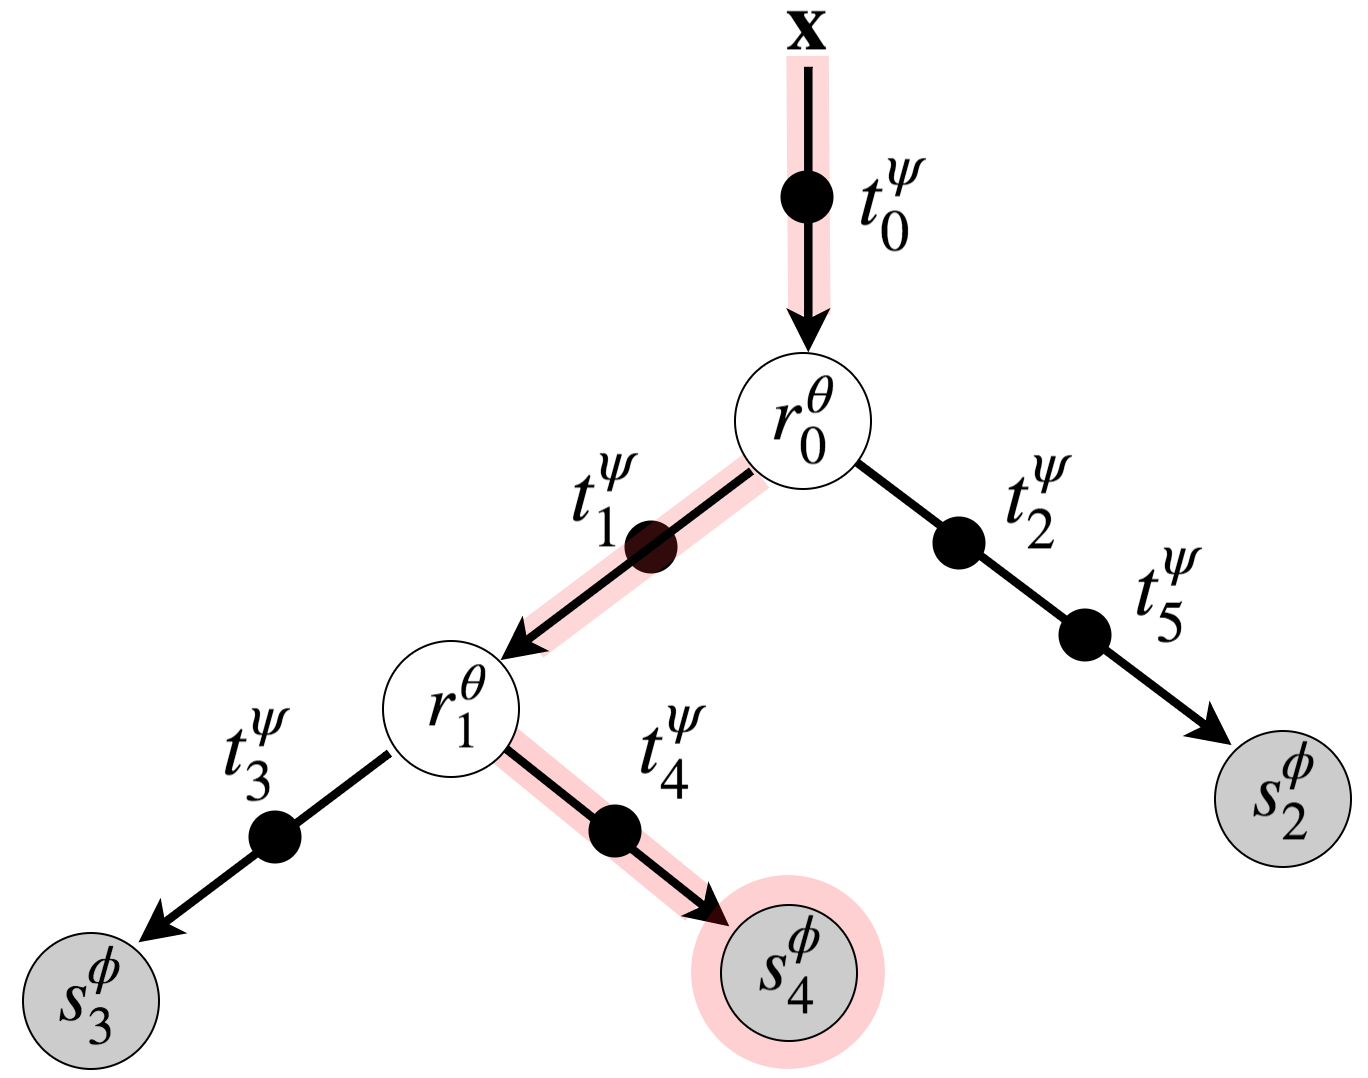
\includegraphics[width=\linewidth]{chapter_7/figures/fig_4_3.png}
	\end{subfigure}
	\hspace{1mm}
	\begin{subfigure}[]{0.52\linewidth}
		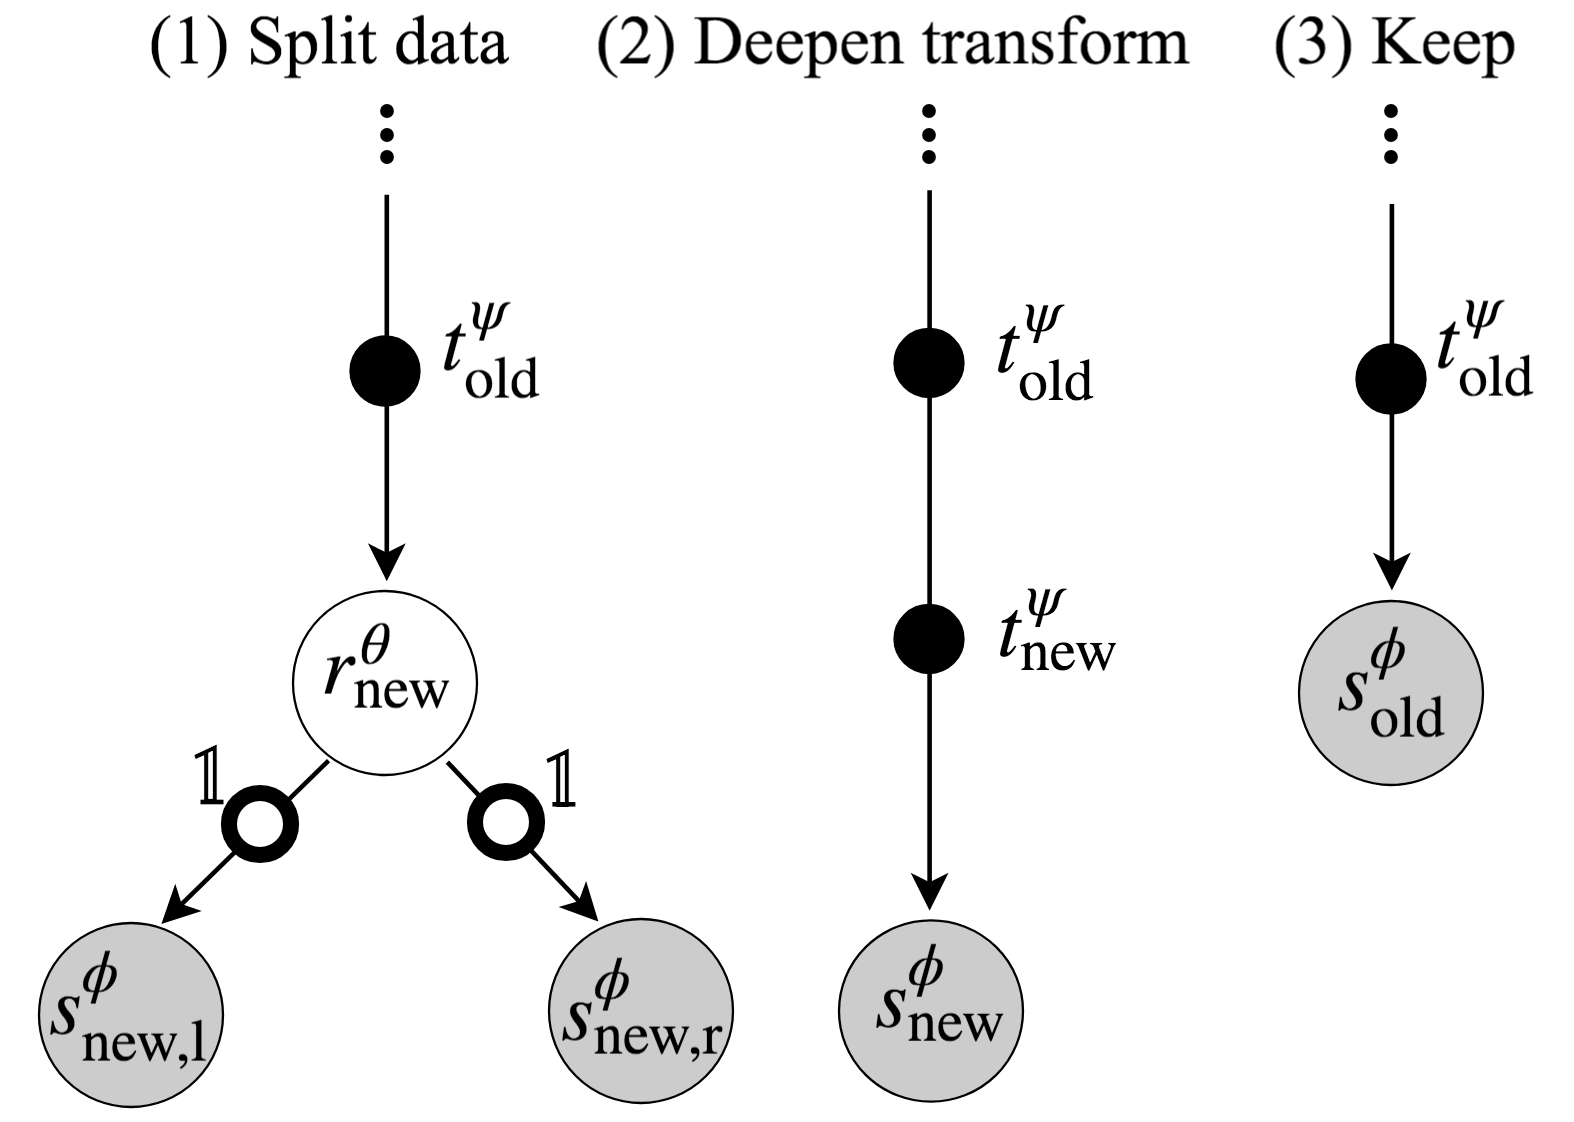
\includegraphics[width=\linewidth]{chapter_7/figures/fig_5_6.png}
	\end{subfigure}
	\caption{\footnotesize \textbf{(Left).} An example ANT. Data is passed through transformers (black circles on edges), routers (white circles on internal nodes), and solvers (gray circles on leaf nodes). The red shaded path shows routing of $\mathbf{x}$ to reach leaf node $4$. Input $\mathbf{x}$ undergoes a series of selected transformations $\mathbf{x}\rightarrow \mathbf{x}^{\boldsymbol{\psi}}_0:=t^{\boldsymbol{\psi}}_0(\mathbf{x})\rightarrow \mathbf{x}^{\boldsymbol{\psi}}_1:=t^{\boldsymbol{\psi}}_1(\mathbf{x}^{\boldsymbol{\psi}}_0) \rightarrow \mathbf{x}^{\boldsymbol{\psi}}_4:=t^{\boldsymbol{\psi}}_4(\mathbf{x}^{\boldsymbol{\psi}}_1)$ and the solver module yields the predictive distribution $p_{4}^{\boldsymbol{\phi}, \boldsymbol{\psi}}(\mathbf{y}):= s^{\boldsymbol{\phi}}_4(\mathbf{x}^{\boldsymbol{\psi}}_4)$. The probability of selecting this path is given by $\pi_{2}^{\boldsymbol{\psi}, \boldsymbol{\theta}}(\mathbf{x}) := r_{0}^{\boldsymbol{\theta}}(\mathbf{x}^{\boldsymbol{\psi}}_0)\cdot(1-r_{1}^{\boldsymbol{\theta}}(\mathbf{x}^{\boldsymbol{\psi}}_1)).$ \textbf{(Right).} Three growth options at a given node: \textit{split data, deepen transform} \& \textit{keep}. The small white circles on the edges denote identity transformers.}
	\label{fig:hierarchy}
\end{figure}

%In this section, we present generalised neural decision trees (ANTs), a form of DTs enhanced with deep, distributed representations. ANTs provide a general framework for combining DTs and NNs, and subsumes prior work in this subject \cite{rota2014neural,kontschieder2015deep} as specific cases. Combined with the optimisation procedure proposed in section \ref{sec:learning}, we will see that ANTs can leverage the differing benefits of the two approaches.
% TODO: Introduce decision trees using the formalism used in the DANT section. Use the DANT section to show the generalisation we introduce.

%a form of decision tree enhanced with deep distributed representation and an efficient mechanism for learning its architecture. The generality of ANTs subsumes the prior work \cite{rota2014neural,kontschieder2015deep,ioannou2016decision} on combining decisions tree and neural networks as specific cases (mode details in section \ref{sec:relatedwork}) and enables to fully leverage the differing benefits of the two approaches. 
%A key difference is the inclusion of transformation operation which enables the representation learning through a series of simple non-linear transforms applied to the input data over the course of traversal down the tree. 
\subsection{Model Topology and Operations}
In short, an ANT is a tree-structured model, characterized by a set of hierarchical partitions of the input space $\mathcal{X}$, a series of nonlinear transformations, and separate predictive models in the respective component regions. More formally, we define an ANT as a pair $(\mathbb{T}, \mathbb{O})$ where $\mathbb{T}$ defines the model topology, and $\mathbb{O}$ denotes the set of operations on it. 

\begin{table}[ht]
	\caption{\footnotesize Primitive module specifications for MNIST, CIFAR-10 and SARCOS datasets. ``conv5-40'' denotes a 2D convolution with 40 kernels of spatial size $5\times5$. ``GAP'', ``FC'', ``LC'' and ``LR'' stand for global-average-pooling, fully connected layer, linear classifier and linear regressor. ``Downsample Freq'' denotes the frequency at which $2\times2$ max-pooling is applied.}
	\label{table:modules}
	%	\vskip 0.15in  % Was 0.15in
	\scriptsize
	\begin{center}
		\centering
		\begin{tabular}{l|c|c|c|c}
			\hline
			%\abovespace
			Model &Router, $\mathcal{R}$ & Transformer, $\mathcal{T}$  & Solver, $\mathcal{S}$& Downsample Freq.\\
			\hline
			ANT-SARCOS& $1 \times \text{FC}$ +\text{Sigmoid} & $1\times$\text{FC}+ \text{tanh} & LR & 0 \\
			\hline
			%\abovespace
			ANT-MNIST-A  & $1\times \text{conv5-40}$ + GAP + $2\times$FC   +\text{Sigmoid} &  $1\times \text{conv5-40}$ + \text{ReLU}&LC& 1 \\
			ANT-MNIST-B& $1\times \text{conv3-40}$ + GAP + $2\times$FC +\text{Sigmoid} & $1\times \text{conv3-40}$ +\text{ReLU} & LC & 2 \\
			ANT-MNIST-C & $1\times \text{conv5-5}$ + GAP + $2\times$FC +\text{Sigmoid}&  $1\times \text{conv5-5}$+\text{ReLU} &LC & 2\\
			\hline
			%\abovespace
			ANT-CIFAR10-A& $2\times \text{conv3-128}$ + GAP + $1\times$FC +\text{Sigmoid} & $2\times \text{conv3-128}$ +\text{ReLU} & LC & 1\\
			ANT-CIFAR10-B & $2\times \text{conv3-96}$ + GAP + $1\times$FC +\text{Sigmoid} &  $2\times \text{conv3-96}$ +\text{ReLU} & LC & 1 \\
			ANT-CIFAR10-C& $2\times \text{conv3-72}$ + GAP + $1\times$FC +\text{Sigmoid} & $2\times \text{conv3-72}$ +\text{ReLU}& GAP + LC & 1 \\
			
% 			\hline
% 			ANT-SARCOS& $1\times$ MLP ($h=128$) & $1\times$ FC ($h=128$) + tanh  & LR & 0
% 			\\
			\hline
		\end{tabular}
	\end{center}
\end{table}

We restrict the model topology $\mathbb{T}$ to be instances of \textit{binary trees}, defined as a set of graphs whose each node is either an internal node or a leaf, and is the child of exactly one parent node, except the root node at the top. We define the topology of a tree as $\mathbb{T} := \{\mathcal{N}, \mathcal{E}\}$ where $\mathcal{N}$ is the set of all nodes, and  $\mathcal{E}$ is the set of edges between them. Nodes with no children are leaf nodes, $\mathcal{N}_{leaf}$, and all others are internal nodes, $\mathcal{N}_{int}$. Every internal node $j \in \mathcal{N}_{int}$ has exactly two children nodes, represented by $\mathrm{left}(j)$ and $\mathrm{right}(j)$. Unlike standard trees, $\mathcal{E}$ contains an edge which connects input data $\mathbf{x}$ with the root node, as shown in Fig.\ref{fig:hierarchy} (Left).

Every node and edge is assigned with operations which acts on the allocated samples of data (Fig.\ref{fig:hierarchy}). Starting at the root, each sample gets transformed and traverses the tree according to the set of operations $\mathbb{O}$. An ANT is constructed based on three primitive modules of differentiable operations: 

\begin{enumerate}
  \item \textbf{Routers}, $\mathcal{R}$: each internal node $j \in \mathcal{N}_{int}$ holds a \textit{router} module, $r_{j}^{\mathbf{\boldsymbol{\theta}}}: \mathcal{X}_j \rightarrow [0, 1] \in \mathcal{R}$, parametrised by $\boldsymbol{\theta}$, which sends samples from the incoming edge to either the left or right child. Here $\mathcal{X}_j $ denotes the representation at node $j$. We use \textit{stochastic routing}, where the decision ($1$ for the left and $0$ for the right branch) is sampled from Bernoulli distribution with mean $r_{j}^{\boldsymbol{\theta}}(\mathbf{x}_j)$ for input $\mathbf{x}_j \in \mathcal{X}_j$. As an example, $r_{j}^{\mathbf{\boldsymbol{\theta}}}$ can be defined as a small CNN.
  
  \item \textbf{Transformers}, $\mathcal{T}$: every edge $e \in \mathcal{E}$ of the tree has one or a composition of multiple \textit{transformer} module(s). Each transformer $t_{e}^{\boldsymbol{\psi}} \in \mathcal{T}$ is a nonlinear function, parametrised by $\boldsymbol{\psi}$, that transforms samples from the previous module and passes them to the next one. For example, $t_{e}^{\boldsymbol{\psi}}$ can be a single convolutional layer followed by ReLU \cite{nair2010rectified}. Unlike in standard DTs, edges transform data and are allowed to ``grow'' by adding more operations (Sec. \ref{sec:learning}), learning ``deeper'' representations as needed.% \textbf{Transformers}, $\mathcal{T}$: every edge $e \in \mathcal{E}$ of the tree (which, say, connects node $j$ with its left child $\mathrm{left}(j)$) has one (or a composition of multiple) \textit{transformer} module(s), $t_{e}^{\boldsymbol{\psi}}: \mathcal{X}_j \rightarrow \mathcal{X}_{\mathrm{left}(j)}  \in \mathcal{T}$, which is a non-linear function,  parametrised by $\boldsymbol{\psi}$, that transforms samples from the previous router and pass them to the next child node. For example, a transformer can be a single convolutional layer followed by ReLU.

  \item \textbf{Solvers}, $\mathcal{S}$: each leaf node $l \in \mathcal{N}_{leaf}$ is assigned to a \textit{solver} module, $s_{l}^{\boldsymbol{\phi}}: \mathcal{X}_l \rightarrow \mathcal{Y}\in \mathcal{S}$, parametrised by $\boldsymbol{\phi}$, which operates on the transformed input data and outputs an estimate for the conditional distribution $p(\mathbf{y}|\mathbf{x})$. For classification tasks, we can define, for example, $s^{\boldsymbol{\phi}}$ as a linear classifier on the feature space $\mathcal{X}_l$, which outputs a distribution over classes. 
\end{enumerate}



Defining operations on the graph $\mathbb{T}$ amounts to a specification of the triplet $\mathbb{O} = (\mathcal{R}, \mathcal{T}, \mathcal{S})$. For example, given image inputs, we would choose the operations of each module to be from the set of operations commonly used in CNNs (examples are given in Tab. \ref{table:modules}).
% In this work, we constrain all operations in each component of $\mathcal{R}, \mathcal{T}, \mathcal{S}$ to take a common form, and in particular, to be a simple building block of standard CNNs. For example, for our MNIST experiments, we specified all transformer modules to take the form of a single convolution layer of fixed size with fixed number of kernels followed by ReLU (other examples are given in Table.\ref{table:modules}).
In this case, every computational path on the resultant ANT, as well as the set of routers that guide inputs to one of these paths, are given by CNNs. Lastly, many existing tree-structured models  \cite{suarez1999globally,irsoy2012soft,laptev2014convolutional,rota2014neural,kontschieder2015deep,frosst2017distilling,xiao2017ndt} are instantiations of ANTs with limitations which we will address with our model (see Sec. \ref{sec:relatedwork} for a more detailed discussion).



% Given a ANT, an input $\mathbf{x}$ stochastically traverses down the tree according to the decisions of routers and undergoes a sequence of selected transformations until it reaches a leaf node where the associated solver module makes the prediction $\mathbf{y}$. 
 
% For example, a standard soft binary decision trees \cite{suarez1999globally} for classification is a specific case where the routers are axis-aligned features, the transformers are identity functions and the solvers are static distribution over classes. The tree model \cite{rota2014neural} instead used multi-layer perceptrons as router modules. Deep Neural Forest \cite{kontschieder2015deep} is an ensemble of neural decision trees, each of which is also an instance of ANT where the whole GoogLeNet architecture except the last fully connected layer is used as the transformer at the root node, and linear classifiers are used for the routers at its internal nodes. However, transformers on the other edges are identity functions and solvers are static class distributions.

% In short, there are two main choices to be made when defining a ANT; (1) the model topology  $\mathbb{T} = \{\mathcal{N}, \mathcal{E}\}$ and (2) the forms of primitive modules $\mathbb{O} = (\mathcal{R}, \mathcal{T}, \mathcal{S})$. In section \ref{sec:learning}, we describe methods for learning $\mathbb{T}$ and $\mathbb{O}$. 

\subsection{Probabilistic Model and Inference}\label{sec:probmodel}
%We now provide a probabilistic interpretation of ANTs and describe possible inference schemes. 
An ANT $(\mathbb{T}, \mathbb{O})$ models the conditional distribution $p(\mathbf{y}|\mathbf{x})$ as a hierarchical mixture of experts (HMEs) \cite{jordan1994hierarchical}, each of which is defined as an NN and is a root-to-leaf path in the tree. Standard HMEs are a special case of ANTs where transformers are the identity function. As a result, the representations within experts are hierarchically shared between similar experts, unlike the independent representations within experts in standard HMEs. In addition, ANTs come with a growth mechanism to determine the number of needed experts and their complexity, as discussed in Sec.~\ref{sec:learning}. 

% Standard HMEs are a specialcase of ANTs where transformers are the identity function.In addition, ANTs come with a growth mechanism to de-termine the number of needed experts and their complexity,as discussed in Sec. 4. A priori it is difficult to determinewhich region of the feature space needs more partitioningor which branches benefit from more nonlinear transfor-mations; ANTs benefit from learning representations thatcan be shared across similar experts, unlike the independentrepresentations within experts in standard HMEs.

%The key difference with traditional HMEs is that the input is not only routed but also transformed within the tree hierarchy (i.e., a standard HMEs is a special case of an ANT with identity transformers).
%As a result, the representations within experts are hierarchically shared and separated, while the experts in standard HMEs are completely independent. In addition, ANTs come with a growth mechanism to determine the number of needed experts and their complexity as discussed in Sec.~\ref{sec:learning}.

Each input to the ANT, $\mathbf{x}$, stochastically traverses the tree based on decisions of routers and undergoes a sequence of transformations until it reaches a leaf node where the corresponding solver predicts the label $\mathbf{y}$. Suppose we have $L$ leaf nodes, the full predictive distribution, with parameters $\Theta = (\boldsymbol{\theta}, \boldsymbol{\psi}, \boldsymbol{\phi})$, is given by
\begin{equation}
p(\mathbf{y}|\mathbf{x}, \Theta)
%= \sum_{\mathbf{z}} p(\mathbf{y}, \mathbf{z}|\mathbf{x}, \boldsymbol{\theta}, \boldsymbol{\psi}, \boldsymbol{\phi}) 
= \sum_{l=1}^{L} 
\underbrace{p(z_l=1|\mathbf{x}, \boldsymbol{\theta}, \boldsymbol{\psi})}_{\text{Leaf-assignment prob. } \pi_{l}^{\boldsymbol{\theta}, \boldsymbol{\psi}}}
\underbrace{p(\mathbf{y}|\mathbf{x}, z_{l}=1,\boldsymbol{\phi}, \boldsymbol{\psi})}_{\text{Leaf-specific prediction. } p_{l}^{\boldsymbol{\phi}, \boldsymbol{\psi}} } \label{eq:2}
\end{equation}

where $\mathbf{z} \in \{0, 1\}^L$ is an $L$-dimensional binary latent variable such that $\sum_{l=1}^{L}z_l = 1$, which describes the choice of leaf node (e.g. $z_l = 1$ means that leaf $l$ is used). Here $\boldsymbol{\theta}, \boldsymbol{\psi}, \boldsymbol{\phi}$ summarise the parameters of router, transformer and solver modules in the tree. The mixing coefficient $\pi_{l}^{\boldsymbol{\theta}, \boldsymbol{\psi}}(\mathbf{x}) := p(z_l=1|\mathbf{x}, \boldsymbol{\psi}, \boldsymbol{\theta})$ quantifies the probability that $\mathbf{x}$ is assigned to leaf $l$ and is given by a product of decision probabilities over all router modules on the unique path $\mathcal{P}_l$ from the root to leaf node $l$:
\begin{equation}
\pi_{l}^{\boldsymbol{\psi}, \boldsymbol{\theta}}(\mathbf{x}) = \prod_{r_{j}^{\boldsymbol{\theta}} \in  \mathcal{P}_l} r_{j}^{\boldsymbol{\theta}}(\mathbf{x}^{\boldsymbol{\psi}}_j)^{\,\mathds{1}_{l \swarrow j}}
\cdot \big{(}1-r_{j}^{\boldsymbol{\theta}}(\mathbf{x}^{\boldsymbol{\psi}}_j)\big{)}^{\,1-\mathds{1}_{l \swarrow j}}
\end{equation}
where $l \swarrow j$ is a binary relation and is only true if leaf $l$ is in the left subtree of internal node $j$, and $\mathbf{x}^{\boldsymbol{\psi}}_j$ is the feature representation of $\mathbf{x}$ at node $j$. Let $\mathcal{T}_j = \{t_{e_1}^{\boldsymbol{\psi}}, ..., t_{e_{n}}^{\boldsymbol{\psi}}\}$ denote the ordered set of the $n$  transformer modules on the path from the root to node $j$, the feature vector $\mathbf{x}^{\boldsymbol{\psi}}_j$ is given by
\begin{equation*}\nonumber
\mathbf{x}^{\boldsymbol{\psi}}_j := 
\Big{(}
t_{e_{n}}^{\boldsymbol{\psi}}
\circ ... \circ
t_{e_{2}}^{\boldsymbol{\psi}}
\circ 		
t_{e_{1}}^{\boldsymbol{\psi}}
\Big{)} (\mathbf{x}).
\vspace{-2mm}
\end{equation*}
On the other hand, the leaf-specific conditional distribution $p_{l}^{\boldsymbol{\phi}, \boldsymbol{\psi}}(\mathbf{y}) := p(\mathbf{y}|\mathbf{x}, z_{l}=1,\boldsymbol{\phi}, \boldsymbol{\psi})$ in \eqref{eq:2}  yields an estimate for the distribution over target $\mathbf{y}$ for leaf node $l$ and is given by its solver's output
 $s_{l}^{\boldsymbol{\phi}}(\mathbf{x}^{\boldsymbol{\psi}}_{\mathrm{parent}(l)})$. 
 
We consider two inference schemes based on a trade-off between accuracy and computation, which we refer to as \textit{multi-path} and \textit{single-path} inference. The multi-path inference uses the \textit{full predictive distribution} given in \eqref{eq:2} as estimate for $p(\mathbf{y}|\mathbf{x})$. However, computing this quantity requires averaging the distributions over all the leaves involving computing all operations at all nodes and edges of the tree, which is expensive for a large ANT. On the other hand, the single-path inference scheme only uses the predictive distribution at the leaf node chosen by greedily traversing the tree in the directions of highest confidence of the routers. This approximation constrains computations to a single path, allowing for more memory- and time-efficient inference.

%We consider two schemes of inference, . First, the \textit{full predictive distribution} given in eq.\eqref{eq:2} is used as the estimate for the target conditional distribution $p(\mathbf{y}|\mathbf{x})$. However, averaging the distributions over all the leaves, weighted by their respective path probabilities, would involve computing all operations at all of the nodes and edges of the tree, which renders the inference expensive for a large ANT. We therefore consider the second scheme where the predictive distribution from the leaf with obtained by greedily traversing the tree in the directions of higher confidence of routers. This approximation constrains computations to a single path on the tree, allowing for more efficient inference.

% Given that the most confident path is known, computation is localised to the path, thus allowing for more efficient inference. 

% However, computing the probabilities of reaching all nodes engages routers at all internal nodes and thus all operational modules on preceding edges, making the path-wise computation almost as expensive as computing the full distribution. We therefore approximately select the most confident path by traversing the tree in the directions of higher confidence of routers. This approximation allows us to constrain the computation to a single path and gets the most confident path in most cases (error rate $0.01\%$) as the router modules generally split data points with high confidence. 

%We therefore also consider an MC approximation where multiple samples of paths are drawn from $\pi_{l}^{\boldsymbol{\theta}, \boldsymbol{\psi}}(\mathbf{x})$ by 
%stochastically traversing the tree according to routers' binary decisions, and the average conditional distributions over the corresponding leaves is used as the final estimate. While marginally reducing the accuracy, this approximation only engages modules on the selected paths and is much more efficient. 

%starting at the root node of the tree, an input $\mathbf{x}$ stochastically traverse down the tree accourding to routers' decisions and undergoes a sequence of selected transformations until it reaches a leaf node where the associated solver module predicts the label $\mathbf{y}$. 
\section{Optimisation}\label{sec:learning}
Training of an ANT proceeds in two stages: 1) \textit{growth phase} during which the model architecture is learned based on \textit{local} optimisation, and 2) \textit{refinement phase} which further tunes the parameters of the model discovered in the first phase based on \textit{global} optimisation. Algorithm~\ref{alg:growth} shows a pseudocode of the training algorithm.

\begin{algorithm}
	\caption{ANT Optimisation}
	\label{alg:growth}
	\footnotesize
	\begin{algorithmic}
		%\Require Topology $\mathbb{T}$, parameters $\theta$
		\State Initialise topology $\mathbb{T}$ and parameters $\mathbb{O}$\Comment{$\mathbb{T}$ is set to a root node with one solver and one transformer}
		\State Optimise parameters in $\mathbb{O}$ via gradient descent on NLL \Comment{Learning root classifier}
		\State Set the root node ``suboptimal"
		
		\While{true} \Comment{Growth of $\mathbb{T}$ begins}
		\State Freeze all parameters $\mathbb{O}$
		\State Pick next ``suboptimal'' leaf node $l\in\mathcal{N}_{leaf}$ in the breadth-first order
		%\State Add (1) linear classifier to $leaf$ and train new parameters?
		\State Add (1) router to $l$ and train new parameters \Comment{Split data}
		\State Add (2) transformer to $l$ and train new parameters\Comment{Deepen transform}
		\State Add (1) or (2) to $\mathbb{T}$ if validation error decreases, otherwise set $l$ to ``optimal''
		\State Add any new modules to $\mathbb{O}$ 
		%\State $b\gets r$
		%\State $r\gets a\bmod b$
		\If{no ``suboptimal'' leaves remain}
		\State Break
		\EndIf
		\EndWhile
		\State Unfreeze and train all parameters in $\mathbb{O}$\Comment{Global refinement with fixed $\mathbb{T}$}
	\end{algorithmic}
\end{algorithm}

 %First, we describe a backpropagation-based algorithm \cite{rumelhart1986learning} for learning parameters in $\mathbb{O}$ given a fixed topology $\mathbb{T}$, which forms the optimisation backbone for both the growth and refinement phases. We then describe a method for learning the model topology, $\mathbb{T}$, and fine-tune it. 

% --------- optimising the parameters in operational modules ------------
\subsection{Loss function: optimising parameters of \texorpdfstring{$\mathbb{O}$}{O}}\label{sec:graddescent}
% \subsection{Loss function: optimising parameters for fixed architecture \texorpdfstring{}{O}}\label{sec:graddescent}
For both phases, we use the negative log-likelihood (NLL) as the common objective function to minimise: 
$$-\text{log }p(\mathbf{Y}|\mathbf{X}, \Theta) = -\sum_{n=1}^N\text{log }(\sum_{l=1}^{L} \pi_{l}^{\boldsymbol{\theta}, \boldsymbol{\psi}}(\mathbf{x}^{(n)})\,
p_{l}^{\boldsymbol{\phi}, \boldsymbol{\psi}}(\mathbf{y}^{(n)}))$$ where $\mathbf{X} = \{\mathbf{x}^{(1)}, ..., \mathbf{x}^{(N)}\}$, $\mathbf{Y} = \{\mathbf{y}^{(1)}, ..., \mathbf{y}^{(N)}\}$ denote the training inputs and targets. As all component modules (routers, transformers and solvers) are differentiable with respect to their parameters $\Theta = (\boldsymbol{\theta}, \boldsymbol{\psi}, \boldsymbol{\phi})$, we can use gradient-based optimisation. Given an ANT with fixed topology  $\mathbb{T}$, we use backpropagation \cite{rumelhart1986learning} for gradient computation and use gradient descent to minimise the NLL for learning the parameters.

%Given a fixed ANT $(\mathbb{T},\mathbb{O})$ and training inputs/targets $\mathbf{X} = \{\mathbf{x}^{(1)}, ..., \mathbf{x}^{(N)}\}$, $\mathbf{Y} = \{\mathbf{y}^{(1)}, ..., \mathbf{y}^{(N)}\}$, we jointly optimise the hierarchical grouping of data to paths on the tree and the associated expert NNs by maximizing the likelihood $p(\mathbf{Y}|\mathbf{X}, \boldsymbol{\theta}, \boldsymbol{\psi}, \boldsymbol{\phi}) = \prod_{n=1}^N\sum_{l=1}^{L} \pi_{l}^{\boldsymbol{\theta}, \boldsymbol{\psi}}(\mathbf{x})\,
%p_{l}^{\boldsymbol{\phi}, \boldsymbol{\psi}}(\mathbf{y}) $. As all the component modules in $\mathbb{O}$ are assumed differentiable with respect to parameters $\Theta = (\boldsymbol{\theta}, \boldsymbol{\psi}, \boldsymbol{\phi})$,  we can use gradient-based optimisation. We use backpropagation for gradient computation and use gradient descent to minimise the negative log-likelihood (NLL): $-\log p(\mathbf{Y}|\mathbf{X},\boldsymbol{\theta}, \boldsymbol{\psi}, \boldsymbol{\phi})$. We employ this scheme for learning parameters in $\mathbb{O}$ in both growth and refinement phases, as explained next. 

% The generalised M-step generates a new estimate of the parameters by taking a gradient ascent on the objective function eq.\eqref{eq:emobj}: $\Theta^{(t+1)} := \Theta^{(t)} + \lambda \frac{\partial}{\partial\Theta}\mathcal{Q}(\Theta|\Theta^{(t)})$ where the gradient is given by the weighted average of component log likelihoods prorated by the previously computed assignment probabilities
% $\frac{\partial}{\partial\Theta}\mathcal{Q}(\Theta|\Theta^{(t)}) = \sum_{n=1}^N \sum_{l=1}^{L} \gamma^{\Theta^{(t)}}(\mathbf{x}^{(n)},\mathbf{y}^{(n)})\, \frac{\partial}{\partial\Theta}\log \pi_{l}^{\boldsymbol{\theta}, \boldsymbol{\psi}}(\mathbf{x^{(n)}})\,
% p_{l}^{\boldsymbol{\phi}, \boldsymbol{\psi}}(\mathbf{y^{(n)}})$.

% \subsubsection{Monte-Carlo approximation of EM}
% The number of leaf nodes can be very large for a deep ANT. The EM-based optimisation requires computation along all possible paths in the given tree structure, incuring an undesirable trade-off between model complexity and training computation. To combat this we propose an Monte-Carlo estimation of the EM objective $\mathcal{Q}(\Theta|\Theta^{(t)})$. 

% In particular, for each input $\mathbf{x}$, we draw multiple samples of destination leaf nodes $\mathcal{N}(\mathbf{x})=\{l_1, ..., l_T\}, \, l_i \sim \pi_{l}^{\boldsymbol{\theta}, \boldsymbol{\psi}}(\mathbf{x})$ by stochastically traversing the tree multiple times and approximate the reaching probability $\pi_{l}^{\boldsymbol{\theta}, \boldsymbol{\psi}}(\mathbf{x})$ for respective leaf nodes by the normalised counting function:
% \begin{equation}
% \widehat{\pi}_{l}^{\boldsymbol{\theta}, \boldsymbol{\psi}}(\mathbf{x}) := \frac{1}{|\mathcal{N}(\mathbf{x})|} \sum_{\tilde{l}\in \mathcal{N}(\mathbf{x}) }\mathbbm{1}[l=\tilde{l}]
% \end{equation}
% We can now form the MC-estimates, $\widehat{\gamma}^{\Theta}(\mathbf{x},\mathbf{y})$ and $\widehat{\mathcal{Q}}(\Theta|\Theta^{(t)})$ of the assigment probability and expected complete-data loglikeilihood by replacing $\pi_{l}^{\boldsymbol{\theta}, \boldsymbol{\psi}}(\mathbf{x})$ terms in eq. \eqref{eq:labelprob} and \eqref{eq:emobj} with $\widehat{\pi}_{l}^{\boldsymbol{\theta}, \boldsymbol{\psi}}(\mathbf{x})$. If a particular computational path is not sampled i.e. $\widehat{\pi}_{l}^{\boldsymbol{\theta}, \boldsymbol{\psi}}(\mathbf{x})=0$, then we do not need to compute the conditional likelihood term $p_{l}^{\boldsymbol{\phi}, \boldsymbol{\psi}}(\mathbf{y})$ at the corresponding leaf node. Therefore, so long as the number of samples $|\mathcal{N}(\mathbf{x})|$ is smaller than the number of leaf nodes, the MC estimates requires less memory and computation than the proposed EM-based iterative optimisation.

% In contrast with the ``soft" assignement of data to different branches in computing $\mathcal{Q}(\Theta|\Theta^{(t)})$, the MC approximation based on sampled computation paths in a tree entails taking a set of sequences of stochastic ``hard" routing decisions where each datum is strictly guided to one branch (left or right) at a time. The need for sampling discrete (binary) decisions means that $\widehat{\mathcal{Q}}(\Theta|\Theta^{(t)})$ is no longer differentiable with respect to the parameters of the router modules $\boldsymbol{\theta}$ (the mean of Bernouli distributions) and so the M-step needs a modification. To this end, we employ a biased path-derivative estimator for Bernouli variables  (``straight-through" estimator) \cite{bengio2013deep} to approximate its expected gradiants. 

% In our experiments, we observed that the number of sampled paths $|\mathcal{N}(\mathbf{x})|$ can be set to $1$ as long as the minibatch size was sufficiently large (e.g. $256$). This simplification renders the E-step redundant (setting $\widehat{\gamma}^{\Theta^{(t)}}(\mathbf{x},\mathbf{y})=1$ for all data points) and reduces the M-step to gradient ascent on the sample conditional log-likelihood
% \begin{equation}\label{eq:emobj}
% \widehat{\mathcal{Q}}(\Theta|\Theta^{(t)}) = \sum_{n=1}^N \log\,p_{l(\mathbf{x^{n}})}^{\boldsymbol{\phi}, \boldsymbol{\psi}}(\mathbf{y}^{(n)}) 
% \end{equation}
% where $l(\mathbf{x^{n}})$ is the sampled leaf node for input $\mathbf{x^{n}}$. We will show in section \ref{sec:experiments} that this aggresive approximation leads to competitive performance in accuracy while significantly reducing the space and time complexity of the original EM algorithm. 
\subsection{Growth phase: learning architecture \texorpdfstring{$\mathbb{T}$}{T}}
We next describe our proposed method for growing the tree $\mathbb{T}$ to an architecture of adequate complexity for the given training data. Starting from the root, we choose one of the leaf nodes in breadth-first order and incrementally modify the architecture by adding computational modules to it. In particular, we evaluate $3$ choices (Fig. \ref{fig:hierarchy} (Right)) at each leaf node; (1)``split data" extends the current model by splitting the node with an addition of a new router; (2) ``deepen transform" increases the depth of the incoming edge by adding a new transformer; (3) ``keep" retains the current model. We then locally optimise the parameters of the newly added modules in the architectures of (1) and (2) by minimising NLL via gradient descent, while fixing the parameters of the previous part of the computational graph. Lastly, we select the model with the lowest validation NLL if it improves on the previously observed lowest NLL, otherwise we execute (3). This process is repeated to all new nodes level-by-level until no more ``split data" or ``deepen transform" operations pass the validation test. 

The rationale for evaluating the two choices is to give the model a freedom to choose the most effective option between ``going deeper'' or splitting the data space. Splitting a node is equivalent to a soft partitioning of the feature space of incoming data, and gives birth to two new leaf nodes (left and right children solvers). In this case, the added transformer modules on the two branches are identity functions. Deepening an edge on the other hand seeks to learn richer representation via an extra nonlinear transformation, and replaces the old solver with a new one. Local optimisation is efficient in time and space; gradients only need to be computed for the parameters of the new parts of the architecture, reducing computation, while forward activations prior to the new parts do not need to be stored in memory, saving space. 

%It is noteworthy that we perform the local optimisation of each `new' architecture for relatively small number of epochs (e.g. up to 20 epochs on MNIST/CIFAR-10). This is motivated by the observation that the performance of a network early in training provides a meaningful indication of performance after convergence \cite{li2017hyperband,brock2017smash}.  We observed that this approach is not only more efficient but also achieves a more accurate model than the standard greedy protocol used in decision tree training where local optimisation is performed until convergence \cite{criminisi2013decision,breiman2001random}. This is presumably because the model is less likely to overfit locally.

\subsection{Refinement phase: global tuning of \texorpdfstring{$\mathbb{O}$}{O}}
Once the model topology is determined in the growth phase, we finish by performing global optimisation to refine the parameters of the model, now with a fixed architecture. This time, we perform gradient descent on the NLL with respect to the parameters of all modules in the graph, jointly optimising the hierarchical grouping of data to paths on the tree and the associated expert NNs. The refinement phase can correct suboptimal decisions made during the local optimisation of the growth phase, and empirically improves the generalisation error (see Sec. \ref{sec:refinement}).
\section{Experiments} 
\label{sec:experiments}
\begin{table*}[t]
	\caption{\small Comparison of performance of different models on SARCOS, MNIST and CIFAR-10. The columns ``Error (multi-path)'' and ``Error (single-path)'' indicate the classification ($\%$) or regression (MSE) errors of predictions based on the multi-path and the single-path inference. The columns ``Params. (multi-path)'' and ``Params. (single-path)'' respectively show the total number of parameters in the model and the average number of parameters used during single-path inference. ``Ensemble Size'' indicates the size of ensemble used. An entry of ``--'' indicates that no value was reported.  Methods marked with \textsuperscript{\textdagger} are from our implementations trained in the same experimental setup. * indicates that the parameters are initialised with a pre-trained CNN.}
	\label{table:mnist_results}
    \centering
    \footnotesize
	\begin{tabular}{|c|l|cc|cc|c|}
		\hline
		%\abovespace\belowspace
		& \multicolumn{1}{c|}{Method}
		& \multicolumn{1}{c}{\thead{\scriptsize Error \\ \scriptsize (multi-path)}}
		& \multicolumn{1}{c}{\thead{\scriptsize Error \\ \scriptsize (single-path)}}
		& \multicolumn{1}{c}{\thead{\scriptsize Params. \\ \scriptsize (multi-path)}}
		& \multicolumn{1}{c|}{\thead{\scriptsize Params. \\ \scriptsize (single-path)}}
		& \multicolumn{1}{c|}{\thead{\scriptsize Ensemble \\ \scriptsize Size}} \\	
		\hline
		\parbox[t]{2mm}{\multirow{12}{*}{\rotatebox[origin=c]{90}{SARCOS}}}
		& Linear regression & 10.693 & N/A & 154 & N/A & 1 \\
		& MLP with 2 hidden layers \cite{zhao2017efficient} & 5.111 & N/A & 31,804 & N/A & 1 \\
		& Decision tree & 3.708 & 3.708 & 319,591 & 25 & 1 \\
		& MLP with 1 hidden layer & 2.835 & N/A & 7,431 & N/A & 1 \\
		& Gradient boosted trees & 2.661 & 2.661 & 391,324 & 2,083 & 7 $\times$ 30 \\
		& MLP with 5 hidden layers & 2.657 & N/A & 270,599 & N/A & 1 \\
		& Random forest & 2.426 & 2.426 & 40,436,840 & 4,791 & 200 \\
		& Random forest & 2.394 & 2.394 & 141,540,436 & 16,771 & 700 \\
		& MLP with 3 hidden layers & 2.129 & N/A & 139,015 & N/A & 1 \\
		&\cellcolor{gray!10}SDT (with MLP routers) &\cellcolor{gray!10} 2.118 &\cellcolor{gray!10} 2.246 &\cellcolor{gray!10} 28,045  &\cellcolor{gray!10} 10,167 &\cellcolor{gray!10} 1\\
		& Gradient boosted trees & 1.444 & 1.444 & 988,256 & 6,808 & 7 $\times$ 100 \\
		&\cellcolor{gray!10}ANT-SARCOS &\cellcolor{gray!10} 1.384 &\cellcolor{gray!10}  1.542 &\cellcolor{gray!10} 103,823  
		&\cellcolor{gray!10} 61,640 &\cellcolor{gray!10} 1\\
		&\cellcolor{gray!10}ANT-SARCOS (ensemble) &\cellcolor{gray!10} 1.226 &\cellcolor{gray!10}  1.372 &\cellcolor{gray!10} 598,280  
		&\cellcolor{gray!10} 360,766 &\cellcolor{gray!10} 8\\
		\hline
		%\abovespace
		\parbox[t]{2mm}{\multirow{14}{*}{\rotatebox[origin=c]{90}{MNIST}}}
        & Linear classifier & 7.91& N/A & 7,840 & N/A&1\\
        & RDT \cite{leon2015policy} & 5.41 & --~~~ & --~~~ & --~~~ & 1\\
		& Random Forests \cite{breiman2001random}& 3.21 & 3.21 & --~~~ & --~~~ &200\\
        & Compact Multi-Class Boosted Trees \cite{ponomareva2017compact} & 2.88 & -- & --~~~  & --~~~ &100 \\
		& Alternating Decision Forest  \cite{schulter2013alternating} & 2.71 & 2.71 & --~~~  & --~~~ &20 \\
		& Neural Decision Tree \cite{xiao2017ndt}& 2.10 & --~~~ &1,773,130 & 502,170&1\\
		&\cellcolor{gray!10}ANT-MNIST-C &\cellcolor{gray!10} 1.62 &\cellcolor{gray!10} 1.68 &\cellcolor{gray!10} 39,670 &\cellcolor{gray!10} 7,956 &\cellcolor{gray!10} 1\\
		& MLP with 2 hidden layers \cite{simard2003best}& 1.40 & N/A & 1,275,200& N/A&1 \\
        & LeNet-5\textsuperscript{\textdagger} \cite{lecun1998gradient} & 0.82 & N/A& 431,000 & N/A & 1\\
		& gcForest \cite{zhou2017deepft} & 0.74 &  0.74 & --~~~  & --~~~  & 500\\
		&\cellcolor{gray!10}ANT-MNIST-B &\cellcolor{gray!10} 0.72 &\cellcolor{gray!10} 0.73 &\cellcolor{gray!10} 76,703 &\cellcolor{gray!10} 50,653 &\cellcolor{gray!10} 1\\
		& Neural Decision Forest \cite{kontschieder2015deep} & 0.70 & --~~ & 544,600 & 463,180 & 10\\
		&\cellcolor{gray!10}ANT-MNIST-A &\cellcolor{gray!10} 0.64 &\cellcolor{gray!10} 0.69 &\cellcolor{gray!10} 100,596&\cellcolor{gray!10} 84,935 &\cellcolor{gray!10} 1\\
		&\cellcolor{gray!10}ANT-MNIST-A (ensemble) &\cellcolor{gray!10} 0.29 &\cellcolor{gray!10} 0.30 &\cellcolor{gray!10} 850,775 &\cellcolor{gray!10} 655,449 &\cellcolor{gray!10} 8 \\
		%		\rowcolor{gray!10} \cellcolor{white} &ANT-MNIST-1 & 0.64 & 0.69 & 100,596& 94,935 & 1\\
		%		\rowcolor{gray!10} \cellcolor{white} &ANT-MNIST-2 & 0.72 & 0.73 &  76,703 & 60,653 & 1\\
		%		\rowcolor{gray!10} \cellcolor{white} &ANT-MNIST-6 & 1.62 & 1.68&  39,670 & 7,956 & 1\\
        & CapsNet \cite{sabour2017dynamic} & 0.25 & --~~ & 8.2M & N/A & 1\\
		\hline
		%\abovespace
		\parbox[t]{2mm}{\multirow{13}{*}{\rotatebox[origin=c]{90}{CIFAR-10}}}                
        & Compact Multi-Class Boosted Trees \cite{ponomareva2017compact} & 52.31 & -- & --~~~  & --~~~ &100 \\
        & Random Forests  \cite{breiman2001random}& 50.17 & 50.17 & --~~~ & --~~~ &2000\\
		& gcForest \cite{zhou2017deepft} & 38.22&  38.22 & --~~~  & --~~~  & 500\\
		& MaxOut \cite{goodfellow2013maxout} & 9.38 & N/A& 6M & N/A & 1\\
        &\cellcolor{gray!10}ANT-CIFAR10-C & \cellcolor{gray!10}9.31 & \cellcolor{gray!10}  9.34& \cellcolor{gray!10} 0.7M &\cellcolor{gray!10} 0.5M & \cellcolor{gray!10}1\\
        &\cellcolor{gray!10}ANT-CIFAR10-B & \cellcolor{gray!10}9.15 & \cellcolor{gray!10}  9.18&  \cellcolor{gray!10}0.9M &\cellcolor{gray!10}0.6M& \cellcolor{gray!10}1\\
		%& dasNet (Stolenga et al., 2014) & 9.22 & N/A & 6M& N/A&1 \\
		& Network in Network \cite{lin2013network} & 8.81 & N/A & 1M  &N/A &1 \\
		& All-CNN\textsuperscript{\textdagger}\cite{springenberg2014striving} & 8.71 & N/A & 1.4M  & N/A &1 \\
		&\cellcolor{gray!10}ANT-CIFAR10-A & \cellcolor{gray!10}8.31 & \cellcolor{gray!10}  8.32 &\cellcolor{gray!10}1.4M&\cellcolor{gray!10}1.0M & \cellcolor{gray!10}1\\
		&\cellcolor{gray!10}ANT-CIFAR10-A (ensemble) & \cellcolor{gray!10}7.71 & \cellcolor{gray!10}  7.79 &\cellcolor{gray!10}8.7M&\cellcolor{gray!10}7.4M & \cellcolor{gray!10}8\\
		&\cellcolor{gray!10}ANT-CIFAR10-A* & \cellcolor{gray!10}6.72 & \cellcolor{gray!10} 6.74 &\cellcolor{gray!10}1.3M&\cellcolor{gray!10}0.8M & \cellcolor{gray!10}1\\
        & ResNet-110 \cite{he2016deep} & 6.43 & N/A & 1.7M  &N/A &1 \\
        & DenseNet-BC (k=24) \cite{huang2017densely} & 3.74 & N/A & 27.2M  &N/A &1 \\
		\hline
		\end{tabular}
\end{table*}

We evaluate ANTs using the SARCOS multivariate regression dataset \cite{vijayakumar2000locally}, and the MNIST \cite{lecun1998gradient} and CIFAR-10 \cite{krizhevsky2009learning} classification datasets. We run ablation studies to show that our different components are vital for the best performance. We then assess the ability of ANTs to automatically learn meaningful hierarchical structures in data. Next, we examine the effects of refinement phase on ANTs, and show that it can automatically prune the tree. Finally, we demonstrate that our proposed training procedure adapts the model size appropriately under varying amounts of labelled data. All of our models are implemented in PyTorch \cite{paszke2017automatic} and is available at  \url{https://github.com/rtanno21609/AdaptiveNeuralTrees}. Full training details, including training times, are provided in Supp.~Sec.~C and D.
% \vspace{-2mm}
% \subsection{Set-up}
% \vspace{-2mm}
% We train ANTs with a range of primitive modules as shown in Tab. \ref{table:modules}. For simplicity, we define the modules based on three types of NN layers: convolutional, global-average-pooling (GAP) and fully-connected (FC). Solver modules are fixed as linear models e.g. logistic regression and linear regression. Router modules are binary classifiers with a sigmoid output. All convolutional and FC layer are followed by ReLU or tanh non-linearities, except in the last layers of solvers and routers. We also apply $2\times2$ max-pooling to feature maps after every $d$ transformer modules where $d$ is the downsample frequency. For the regression experiment, hidden layers in the baseline MLPs, routers and transformers contain 256 units. We balance the number of parameters in the router and transformer modules to be of the same order of magnitude to avoid favouring either partitioning the data or learning more expressive features. In the growth phase the parameters for the new modules are trained until convergence, as determined by patience-based early stopping on the validation set. The patience level is an important hyperparameter tuned based on the validation set, and a quantitative evaluation of its effect on performance is given in Supp.~Sec.~E. Full training details, including training times, are provided in Supp.~Sec.~C and D, with details of ANT ensembles provided in Supp.~Sec.~I.

\subsection{Model Performance}
We compare the performance of ANTs (Tab. \ref{table:modules}) against a range of DT and NN models (Tab. \ref{table:mnist_results}), where notably the relative performance of these two classes of models differs between datasets. ANTs inherit from both and achieve the lowest error on SARCOS, and perform favourably on MNIST and CIFAR-10. In general, DT methods without feature learning, such as RFs \cite{breiman2001random,zhou2017deepft} and GBTs \cite{ponomareva2017compact}, perform poorly on image classification tasks \cite{krizhevsky2009learning}. In comparison with CNNs without shortcut connections \cite{lecun1998gradient,goodfellow2013maxout,lin2013network,springenberg2014striving}, different ANTs balance between stronger performance with comparable numbers of trainable parameters, and comparable performance with smaller amount of parameters. At the other end of the spectrum, state-of-the-art NNs \cite{sabour2017dynamic,huang2017densely} contain significantly more parameters.
%On these image datasets, ANTs outperform other NNs with similar parameter counts, but fail to reach the performance of state-of-the-art models \cite{sabour2017dynamic,huang2017densely} which contain an order of magnitude more parameters.

\textbf{Conditional computation:} Tab.\ref{table:mnist_results} compares the errors and number of parameters of different ANTs for both multi-path and single-path inference schemes. While reducing the number of parameters (from Params (multi-path) to Params (single-path)) across all ANT models, we observe only a small difference in error (between Error (multi-path) and Error (single-path)), with the largest deviations being $0.06\%$ for classification and $0.158$ for regression. In addition, Supp.Sec.~H shows that the single-path inference reduces FLOPS. This means that single-path inference gives an accurate approximation of the multi-path inference, while being more efficient to compute. This close approximation comes from the confident splitting probabilities of routers, being close to 0 or 1 (see blue histograms in Fig. \ref{fig:learnedmodel}(b)).

% The latter would, however, require computing the probabilities of reaching all the nodes of the tree, which engages all operational modules except the solvers and thus is almost as expensive as computing the full distribution. We therefore instead approximate the most confident path by traversing the tree in the directions of higher confidence of routers. This approximation allowes us to constrain the computation to a single path and holds true in most cases (error rate $0.01\%$) as the router modules guide data points with high confidence.

% \textbf{Patience-based local optimisation:} in the growth phase the parameters for the new modules are trained until convergence, as determined by patience-based early stopping on the validation set. We observe that very low or high patience levels result in new modules underfitting or overfitting locally, thus preventing meaningful further growth% and leading to differences of up to 10\% in validation accuracy.
% . We tuned this hyperparameter using the validation sets, and set the patience level to $5$, which produced consistently good performance on both MNIST and CIFAR-10 datasets across different specifications of primitive modules. A quantitative evaluation is given in the supplementary (Sec.~E).

%in the growth phase, the number of optimisation steps spent for the trial of each new model affects the discovered architecture, and consequently the classification performance. If too few steps of optimisation are performed, then the added modules would not be tuned enough. On the other hand, if too many optimisation steps are taken, this causes the added component to overfit locally. Both extremes prevent the model from making a meaningful further growth. We thus employed patience based early-stopping, and selected the best patience level based on validation accuracy on both MNIST and CIFAR-10. A quantitative evaluation is given in the supplementals.
\textbf{Ablation study:} we compare the predictive errors of different variants of ANTs in cases where the options for adding transformer or router modules are disabled (see Tab. \ref{tab:ablationstudy}). In the first case, the resulting models are equivalent to SDTs \cite{suarez1999globally} or HMEs \cite{jordan1994hierarchical} with locally grown architectures, while the second case is equivalent to standard CNNs, grown adaptively layer by layer. We observe that either ablation consistently leads to higher errors across different module configurations on all three datasets, justifying the combination of feature learning and hierarchical partitioning in ANTs.

\textbf{SARCOS multivariate regression:} Tab.~\ref{table:mnist_results} shows that ANT-SARCOS outperforms all other methods in mean squared error (MSE) with the full set of parameters. With the single-path inference, GBTs performs slightly better than a single ANT while requiring fewer parameters. We note that the top 3 methods are all tree-based, with the third best method being an SDT (with MLP routers). On the other hand, ANT and GBTs outperform the best standard NN model with less than a half of the parameter count. This highlights the value of hierarchical clustering for predictive performance and inference speed. Meanwhile, we still reap the benefits of representation learning, as shown by both ANT-SARCOS and the SDT (which is a specific form of ANT with identity transformers) requiring fewer parameters than the best-performing GBT configuration. Finally, we note that deeper NNs (5 vs. 3 hidden layers) can overfit on this small dataset, which makes the adaptive growth procedure of tree-based methods ideal for finding a model that exhibits good generalisation. 



%Tab.~\ref{table:mnist_results} shows that ANT-SARCOS outperforms all other methods in mean squared error (MSE) with the full set of parameters. With the single-path inference, GBTs performs slightly better than a single ANT while requiring fewer parameters. An ensemble of ANTs achieves the best results over all in both multi- and single-path inference. We note that the top 3 performing methods are all tree-based, with the third best method being an SDT (with MLP routers). %Despite the proliferation of deep-learning-based methods for highly structured data such as images and text, GBTs and RFs can still outperform them on other sorts of data, such as we have here. 
%This highlights the value of hierarchical clustering of the input space for predictive performance. Meanwhile, we still reap the benefits of representation learning, as shown by both ANT-SARCOS and the SDT (which is a specific form of ANT with identity transformers) requiring fewer parameters than the best-performing GBT configuration. Finally, we note that deeper NNs (5 vs. 3 hidden layers) can overfit on this small dataset, which makes the adaptive growth procedure of tree-based methods ideal for finding a model that exhibits good generalisation.

%Tab.~\ref{table:mnist_results} shows that the top 3 models are all tree-based, with NDT, GBTs and ANT achieving the lowest MSE. ANT requires less than a half of what’s required for the best standard NN model. On the other hand, Gradient Boosted trees only need a magnitude less parameters. We should however note that the total number of parameters for standard trees models are significantly larger than that of an ANT. All in all, ANT achieves the best accuracy on SARCOS beating both standard NNs and standard tree-based methods. Secondly, in terms of computational efficiency, ANTs is somewhere between NNs and GBTs. This highlights the value of hierarchical clustering of the input space for both predictive accuracy and speed. 

\textbf{MNIST digit classification:} we observe that ANT-MNIST-A outperforms state-of-the-art GBT \cite{ponomareva2017compact} and RF \cite{zhou2017deepft} methods in accuracy. This performance is attained despite the use of a single tree, while RF methods operate with ensembles of classifiers (the size shown in Tab. \ref{table:modules}). In particular, the NDF \cite{kontschieder2015deep} has a pre-specified architecture where LeNet-5 \cite{lecun1998gradient} is used as the root transformer module, and $10$ trees of fixed depth $5$ are built on this base features. On the other hand, ANT-MNIST-A is constructed in a data-driven manner from primitive modules, and displays an improvement over the NDF both in terms of accuracy and number of parameters. In addition, reducing the size of convolution kernels (ANT-MNIST-B) reduces the total number of parameters by $25\%$ and the path-wise average by almost $40\%$ while only increasing the error by $< 0.1\%$.

We also compare against the LeNet-5 CNN \cite{lecun1998gradient}, comprised of the same types of operations used in our primitive modules (i.e. convolutional, max-pooling and FC layers). For a fair comparison, the network is trained with the same protocol as that of the ANT refinement phase, achieving an error rate of $0.82\%$. Both ANT-MNIST-A and ANT-MNIST-B attain better accuracy with a smaller number of parameters than LeNet-5. The current state-of-the-art, capsule networks (CapsNets) \cite{sabour2017dynamic}, have more parameters than ANT-MNIST-A by almost two orders of magnitude.\footnote{Notably, CapsNets also feature a routing mechanism, but with a significantly different mechanism and motivation.} By ensembling ANTs, we can reach similar performance ($0.29\%$ versus $0.25\%$) with an order of magnitude less parameters (see Supp.Sec.~H).

Lastly, we highlight the observation that ANT-MNIST-C, with the simplest primitive modules, achieves an error rate of $1.68\%$ with single-path inference, which is significantly better than that of the linear classifier ($7.91\%$), while engaging almost the same number of parameters ($7,956$ vs. $7,840$) on average. To isolate the benefit of convolutions, we took one of the root-to-path CNNs on ANT-MNIST-C and increased the number of kernels to adjust the number of parameters to the same value. We observe a higher error rate of $3.55\%$, which indicates that while convolutions are beneficial, data partitioning has additional benefits in improving accuracy. This result demonstrates the potential of ANT growth protocol for constructing performant models with lightweight inference. See Sec.~G in the supplementary materials for the architecture of ANT-MNIST-C.

\begin{table}[t]
	\caption{\footnotesize Ablation study on regression (MSE) and classification ($\%$) errors. ``CNN'' refers to the case where the ANT is grown without routers while ``SDT/HME'' refers to the case where transformer modules on the edges are disabled.} \label{tab:ablationstudy}
	\footnotesize
    \center
	\begin{tabular}{|l|ccc|ccc|}
		\hline
		\multicolumn{1}{|c}{\textbf{Model}} &  \multicolumn{3}{|c|}{\textbf{Error (multi-path)}} & \multicolumn{3}{c|}{\textbf{Error (single-path)}}  \\
			& ANT & CNN & HME & ANT & CNN & HME  \\
			& (default) & (no $\mathcal{R}$) & (no $\mathcal{T}$) & (default) & (no $\mathcal{R}$) & (no $\mathcal{T}$) \\
		\hline
		SARCOS &1.38 & 2.51 & 2.12 &1.54 & 2.51 & 2.25 \\
		MNIST-A &0.64 & 0.74 & 3.18 &0.69 & 0.74 & 4.19  \\
	    MNIST-B &0.72 & 0.80 & 4.63 &0.73 & 0.80 & 3.62\\
        MNIST-C &1.62 & 3.71 & 5.70 &1.68 & 3.71 & 6.96 \\
		CIFAR10-A &8.31 & 9.29 & 39.29   & 8.32 & 9.29 & 40.33 \\
        CIFAR10-B &9.15 & 11.08 & 43.09 & 9.18 & 11.08 & 44.25 \\
        CIFAR10-C &9.31 & 11.61 & 48.59 & 9.34 & 11.61 & 50.02 \\
		\hline
	\end{tabular}
\end{table}

\textbf{CIFAR-10 object recognition:} we see that ANTs largely outperform the state-of-the-art DT method, gcForest \cite{zhou2017deepft}, achieving over 90\% accuracy, demonstrating the benefit of representation learning in tree-structured models. Secondly, with fewer number of parameters in single-path inference, ANT-CIFAR-A achieves higher accuracy than CNN models without shortcut connections \cite{goodfellow2013maxout,lin2013network,springenberg2014striving} that held the state-of-the-art performance in respective years. With simpler primitive modules we learn more compact models (ANT-MNIST-B and -C) with a marginal compromise in accuracy. In addition, initialising the parameters of transformers and routers from a pre-trained single-path CNN further reduced the error rate of ANT-MNIST-A by 20\% (see ANT-MNIST-A* in Tab. \ref{table:mnist_results}), indicating room for improvement in our proposed optimisation method.

Shortcut connections \cite{fahlman1990cascade} have recently lead to leaps in performance in deep CNNs \cite{he2016deep,huang2017densely}. We observe that our best network, ANT-MNIST-A*, has a comparable error rate and half the parameter count (with single-path inference) to the best-performing residual network, ResNet-110 \cite{he2016deep}. Densely connected networks leads to better accuracy, but with an order of magnitude more parameters \cite{huang2017densely}. We expect shortcut connections to improve ANT performance, and leave integrating them to future work.

%We note that the comparison is limited to NNs of up to 15 layers with same set of operations (e.g. convolutions, GAP and FC layers) and linear architectures. For simplicity, we did not consider primitive modules based on more recent models such as residual \cite{he2016deep} and dense connections \cite{huang2017densely}, which present lower error rates than our best result. However, ANTs are ameable to these advances.

%\textcolor{red}{we compare variants of ANTs with module specifications in Tab. \ref{table:modules} against modern NN models, and results are summarized in the bottom half of Tab.\ref{table:mnist_results}. We limit our comparison to NNs of up to $15$ layers with the same set of simple operations and linear architectures. In particular, we choose All-CNN as the baseline which reports the lowest error among the comparison targets and is the closest in terms of constituent operations (convolutional, GAP and FC layers). For a fair comparison, we train our reimplementation of the model in the same experimental set-up as the refinement phase of ANT training, and report the new performance. We also apply batch normalization \cite{ioffe2015batch} after every convolutional layer both in ANT modules, and All-CNN, as it improved convergence and accuracy.} We observe that our growth protocol can discover an architecture (ANT-CIFAR10-A) which attains lower error than All-CNN while retaining a similar number of parameters in total, and $20\%$ less for path-wise inference. Simpler modules lead to more compact models (ANT-CIFAR10-B and C) with a marginal compromise in accuracy.
%\textcolor{blue}{It should be noted that our framework is amenable to more recent advances in deep learning, such as residual learning \cite{he2016deep} and dense connections \cite{huang2017densely}, which all present lower error rates than our best result, but can also be integrated into ANT modules. We leave an investigation of these more complex “primitives” for future work.}

%\subsection{Learned hierarchical structures}
\subsection{Interpretability}
The growth procedure of ANTs is capable of discovering hierarchical structures in the data that are useful to the end task. Without any regularization imposed on routers, the learned hierarchies often display strong specialisation of paths to certain classes or categories of data on both the MNIST and CIFAR-10 datasets. Fig. \ref{fig:learnedmodel} (a) displays an example with particularly ``human-interpretable'' partitions e.g. man-made versus natural objects, and road vehicles versus other types of vehicles. It should, however, be noted that human intuitions on relevant hierarchical structures do not necessarily equate to optimal representations, particularly as datasets may not necessarily have an underlying hierarchical structure, e.g., MNIST. Rather, what needs to be highlighted is the ability of ANTs to learn when to share or separate the representation of data to optimise end-task performance, which gives rise to automatically discovering such hierarchies. To further attest that the model learns a meaningful routing strategy, we also present the test accuracy of the predictions from the leaf node with the smallest reaching probability in Supp.~Sec.~F. We observe that using the least likely ``expert'' leads to a substantial drop in classification accuracy. In addition, most learned trees are unbalanced. This property of adaptive computation is plausible since certain types of images may be easier to classify than others, as seen in prior work \cite{Figurnov2017SpatiallyAC}.

\subsection{Effect of global refinement} \label{sec:refinement}
\begin{figure*}[t!]
	\center
	\begin{subfigure}[t]{0.9\linewidth}
		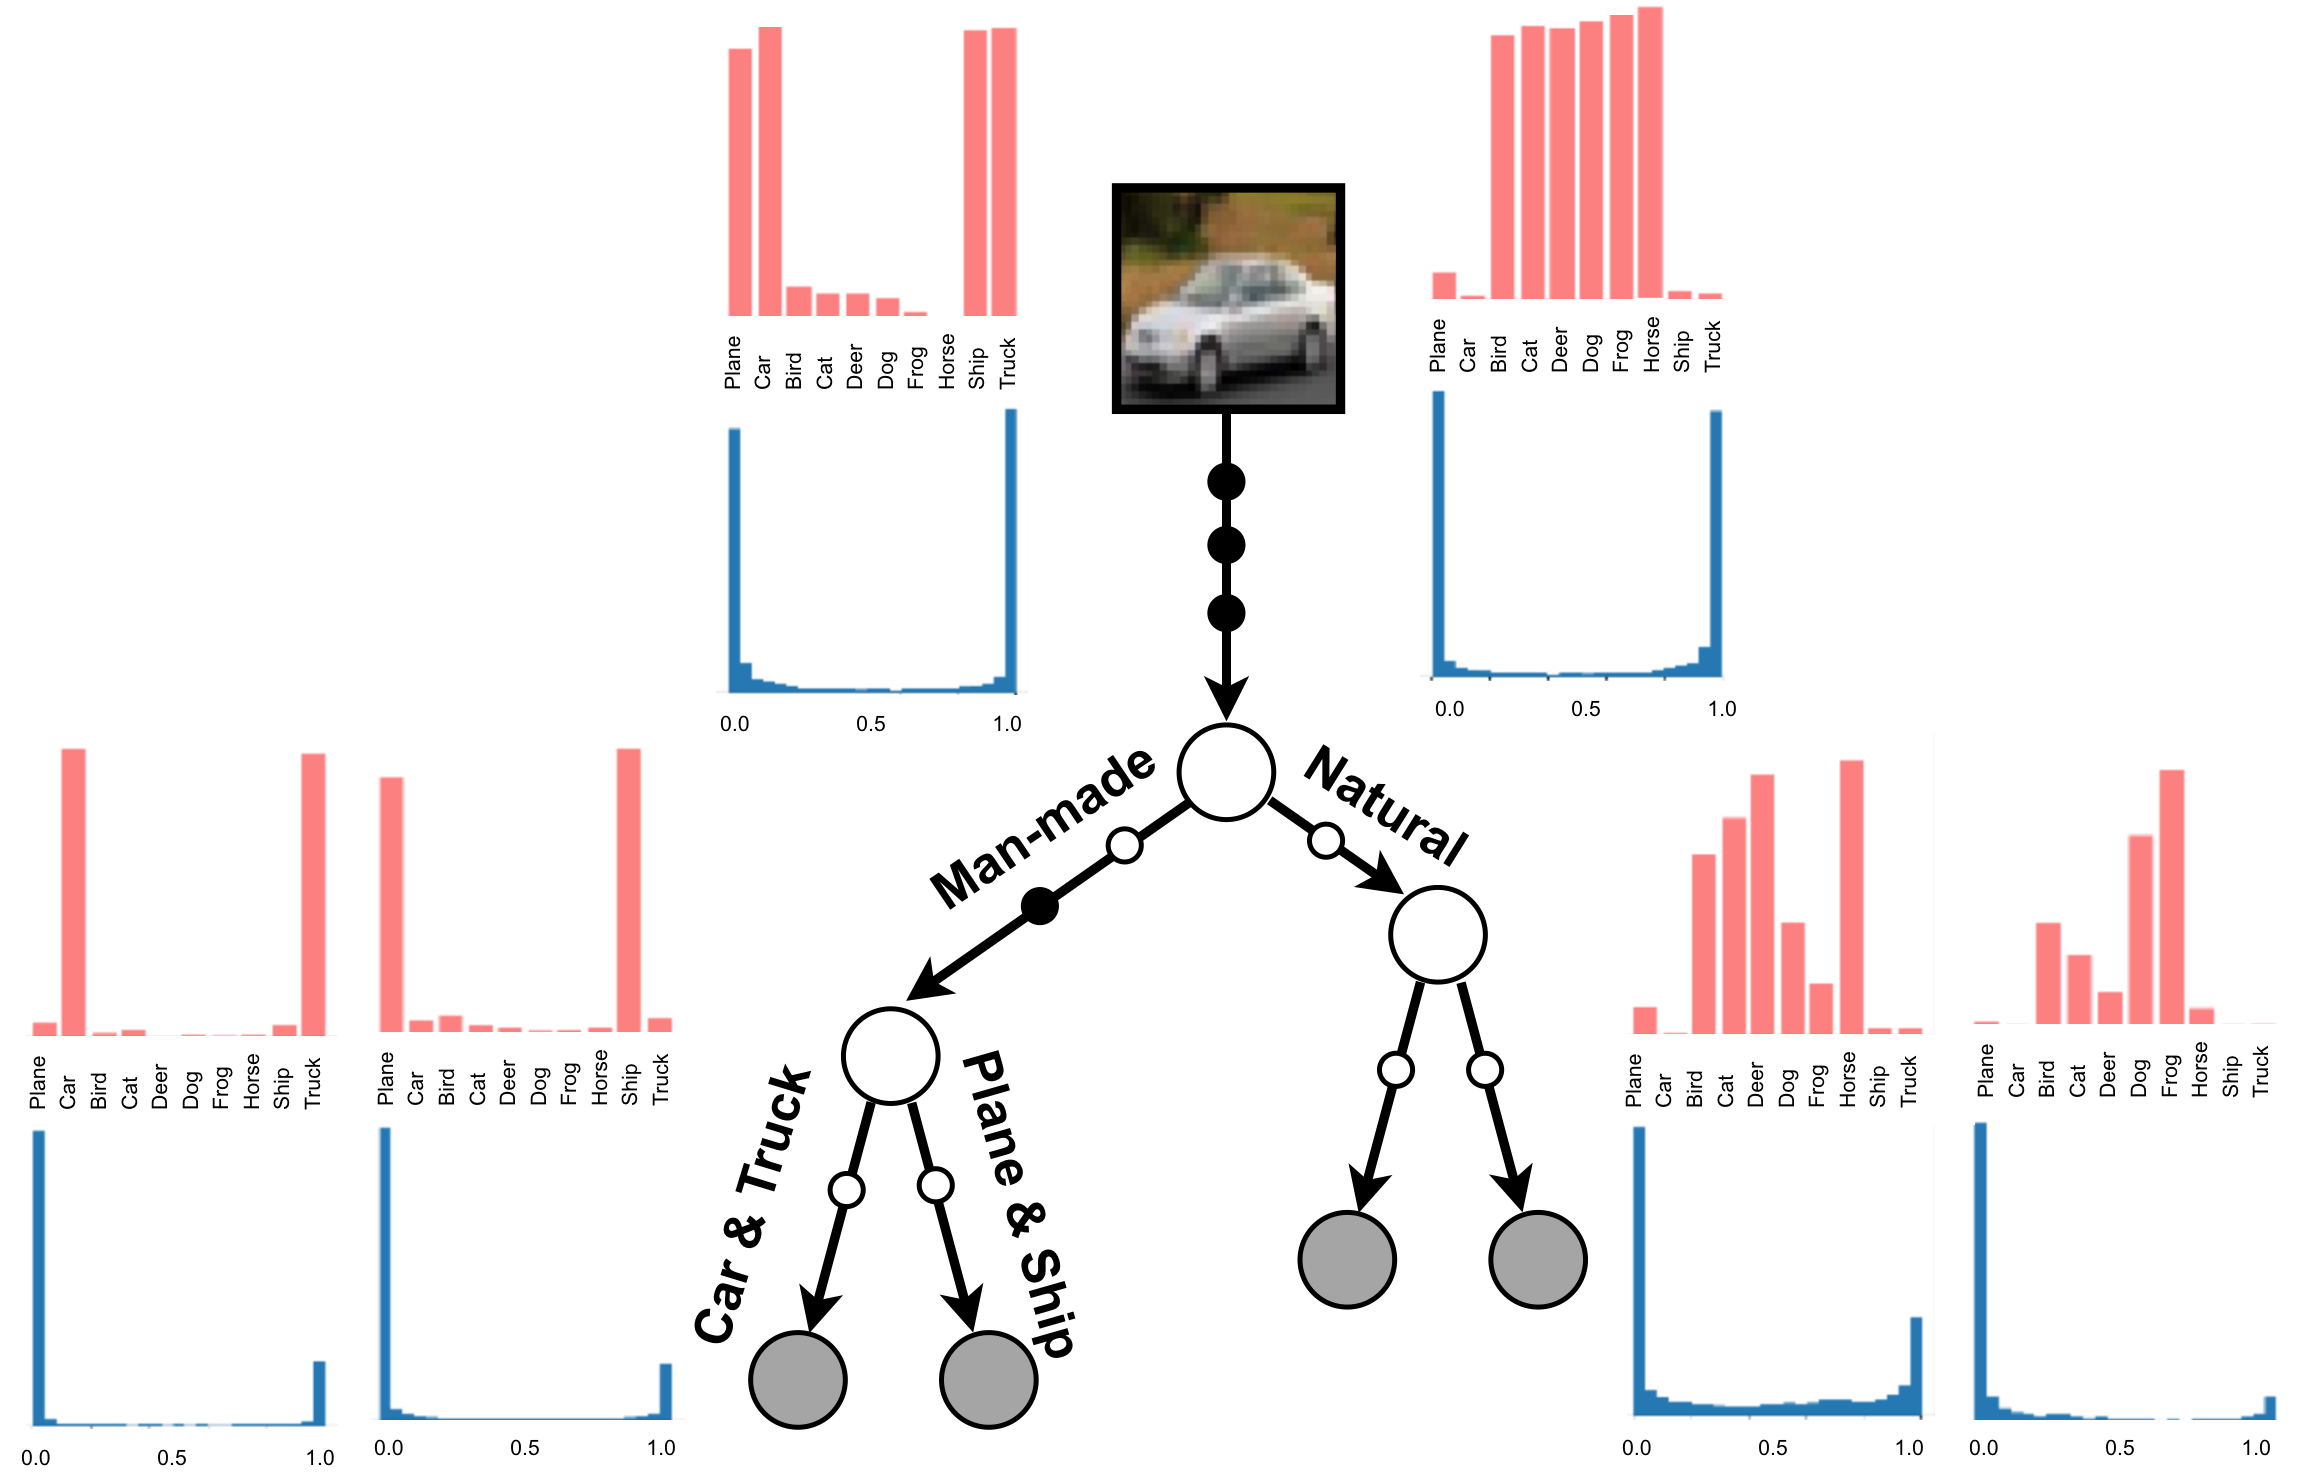
\includegraphics[width=\linewidth]{chapter_7/figures/fig_7_9.png}
		%\label{fig:ch5:active}
		\vspace{-6mm}
		\caption{Before refinement}
	\end{subfigure}
	\hspace{4.66mm}
	\begin{subfigure}[t]{0.9\linewidth}
		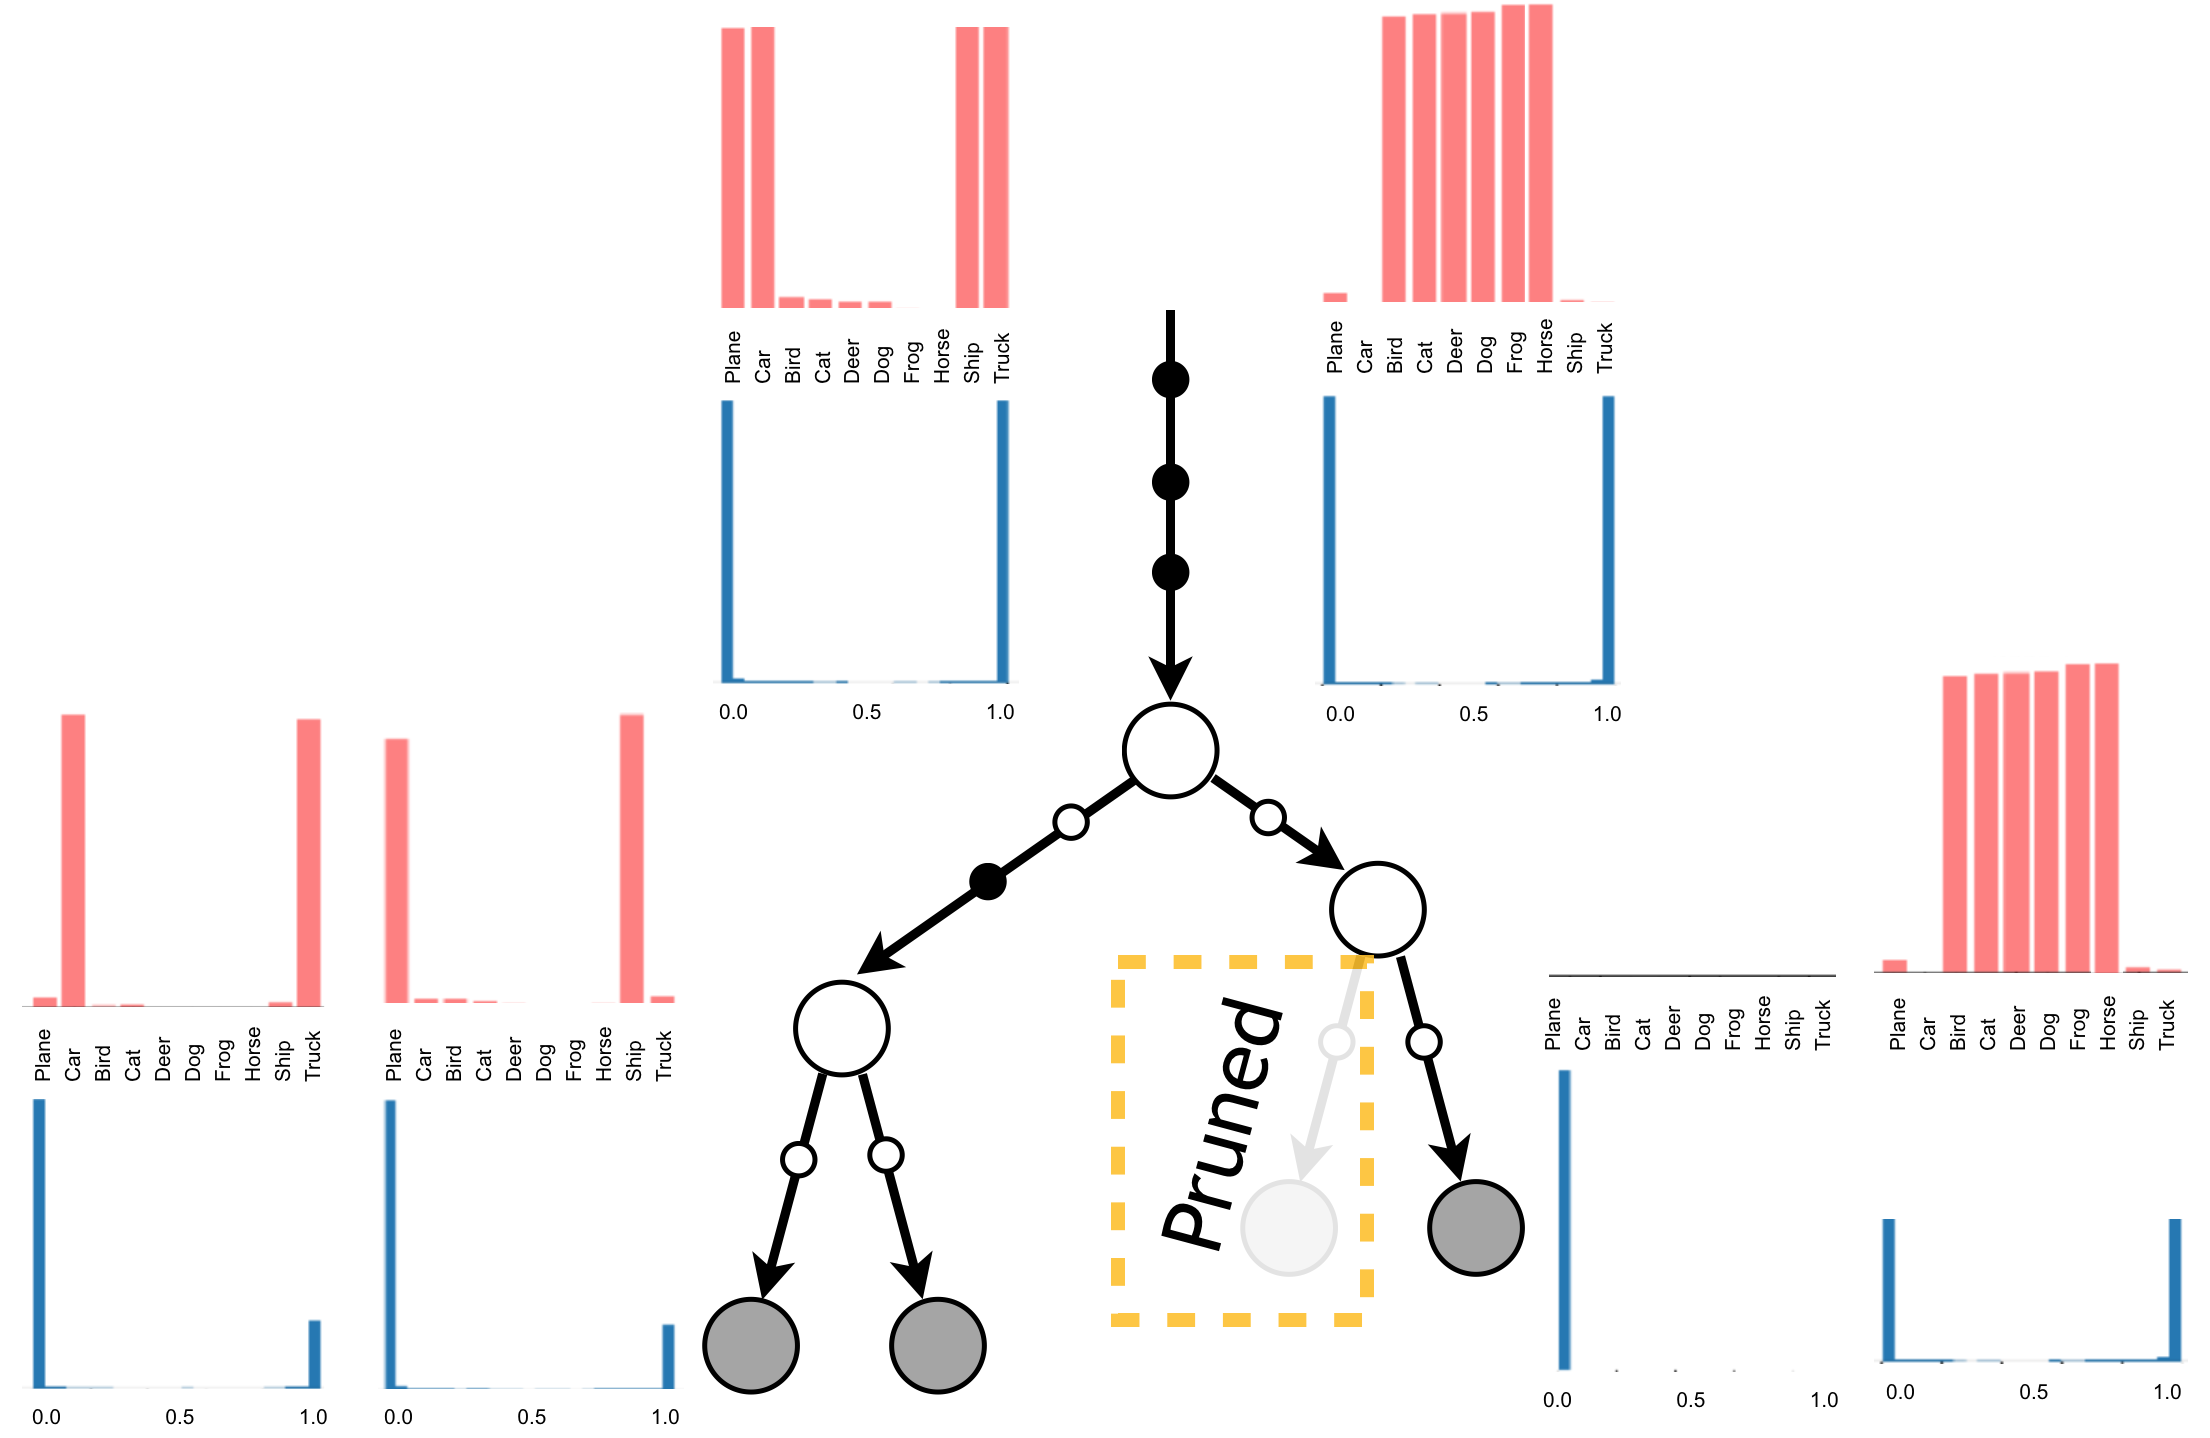
\includegraphics[width=\linewidth]{chapter_7/figures/fig_7_10.png}
		%\label{fig:ch5:active2}
		\vspace{-6mm}
		\caption{After refinement}
	\end{subfigure}
	\caption{\small Visualisation of class distributions (red) and path probabilities (blue) computed over the whole test set at respective nodes of an example ANT (a) before and (b) after the refinement phase. (a) shows that the model captures an interpretable hierarchy, grouping semantically similar images on the same branches. (b) shows that the refinement phase polarises path probabilities, pruning a branch.}
	\label{fig:learnedmodel}
\end{figure*}

\begin{figure}[t!]
	\centering
	\begin{subfigure}[t]{0.48\linewidth}
		\caption{}
		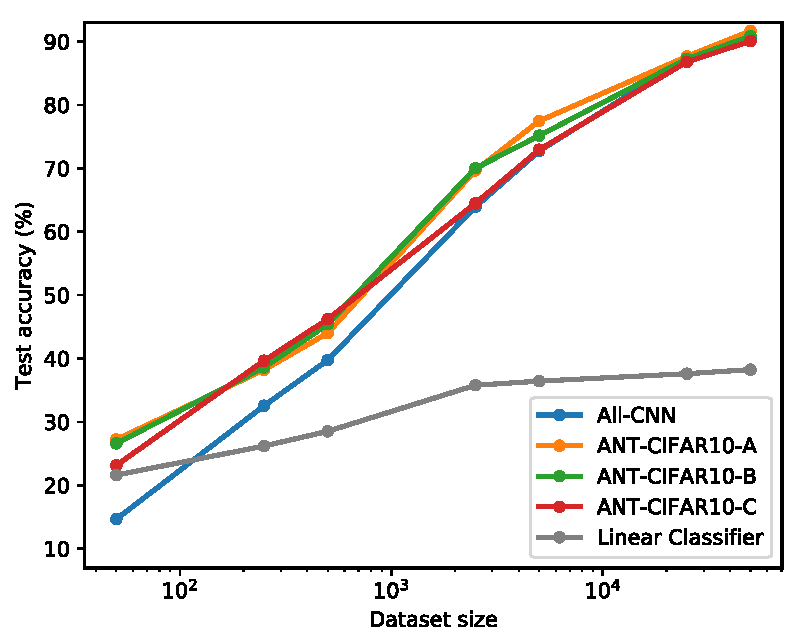
\includegraphics[width=\linewidth]{chapter_7/figures/fig_1_2.pdf}
		%\label{fig:ch5:active}
	\end{subfigure}
	\hspace{0mm}
	\begin{subfigure}[t]{0.50\linewidth}
		\caption{}
		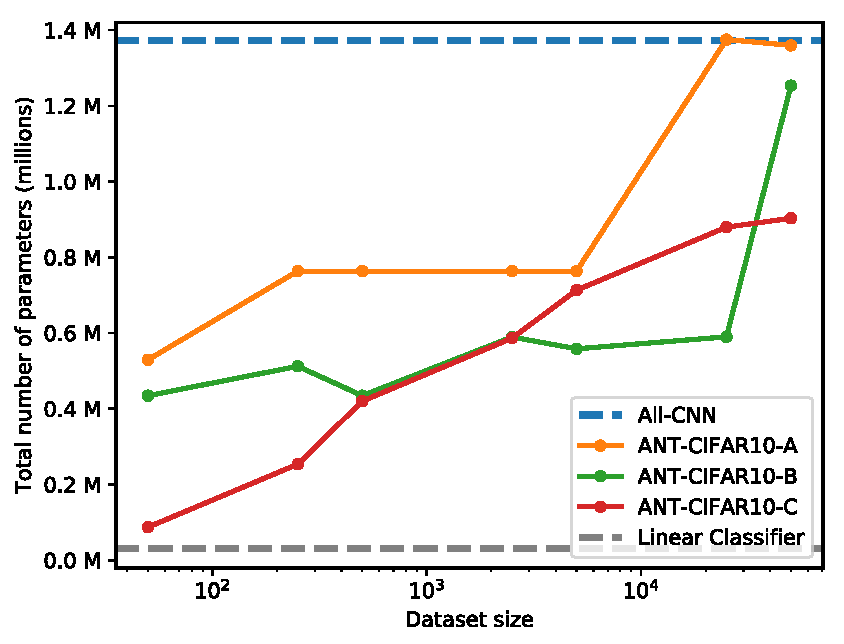
\includegraphics[width=\linewidth]{chapter_7/figures/fig_2_2.pdf}
		%\label{fig:ch5:active2}
	\end{subfigure}
	\hspace{0mm}
	\begin{subfigure}[t]{0.52\linewidth}
		\caption{}
		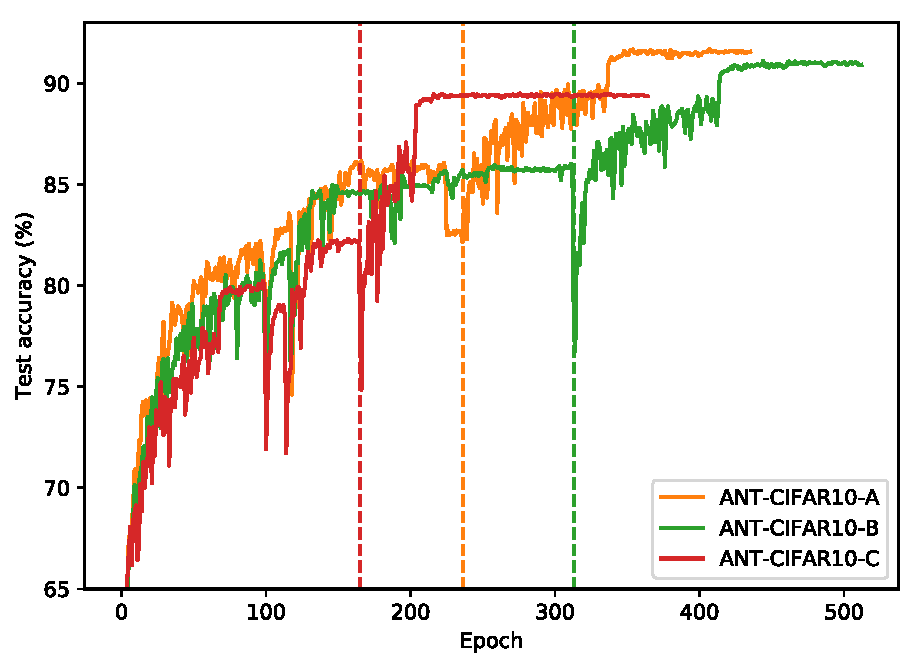
\includegraphics[width=\linewidth]{chapter_7/figures/fig_3_2.pdf}
		%\label{fig:ch5:active2}
	\end{subfigure}
	\caption{\small (a) Test accuracy on CIFAR-10 of ANTs for varying amounts of training data. (b) The complexity of the grown ANTs increases with dataset size. (c) Refinement improves generalisation; the dotted lines show where the refinement phase starts.}
	\label{fig:cifar10}
\end{figure}

We observe that global refinement phase improves the generalisation error. Fig. \ref{fig:cifar10} (Right) shows the generalisation error of various ANT models on CIFAR-10, with vertical dotted lines indicating the epoch when the models enter the refinement phase. As we switch from optimising parts of the ANT in isolation to optimising all parameters, we shift the optimisation landscape, resulting in an initial drop in performance. However, they all consistently converge to higher test accuracy than the best value attained during the growth phase. This provides evidence that refinement phase remedies suboptimal decisions made during the locally-optimised growth phase. In many cases, we observed that global optimisation polarises the decision probability of routers, which occasionally leads to the effective ``pruning" of some branches. For example, in the case of the tree shown in Fig. \ref{fig:learnedmodel}(b), we observe that the decision probability of routers are more concentrated near 0 or 1 after global refinement, and as a result, the empirical probability of visiting one of the leaf nodes, calculated over the validation set, reduces to 0.09\%---meaning that the corresponding branch could be pruned without a negligible change in the network's accuracy. The resultant model attains lower generalisation error, showing the pruning has resolved a suboptimal partioning of data. 
%We emphasise that this is a consequence of global fine-tuning, and does not involve additional algorithms that would be used to prune or compress standard NNs.

%We observe that global refinement step improves the generalisation error. Fig. \ref{fig:cifar10} (right) shows the generalisation error on CIFAR-10 of various ANT models, with vertical dotted lines indicating the epoch when the models enter the refinement phase. While the models initially undergo a steep drop in performance, they all consistently converge to higher test accuracy than the best value attained during the growth phase. This provides evidence that global optimisation remedies suboptimal decisions made during the locally optimised growth phase. For example, refinement tends to polarize the decisions of routers, which can allow some branches to be pruned (see Fig. \ref{fig:learnedmodel}); this improves generalisation, indicating resolvement of suboptimal partitioning of data. 


\subsection{Adaptive model complexity}
Overparametrised models, trained without regularization, are vulnerable to overfitting on small datasets. Here we assess the ability of our proposed ANT training method to adapt the model complexity to varying amounts of labelled data. We run classfication experiments on CIFAR-10 and train three variants of ANTs, All-CNN \cite{springenberg2014striving} and linear classifier on subsets of the dataset of sizes 50, 250, 500, 2.5k, 5k, 25k and 45k (the full training set). Here we choose All-CNN as the baseline as it has similar number of parameters when trained on the full dataset and is the closest in terms of constituent operations (convolutional, GAP and FC layers).
Fig.\ref{fig:cifar10} (Left) shows the corresponding test performances. The best model is picked based on the performance on the same validation set of 5k examples as before. As the dataset gets smaller, the margin between the test accuracy of the ANT models and All-CNN/linear classifier increases (up to $13\%$). Fig. \ref{fig:cifar10} (Middle) shows the model size of discovered ANTs as the dataset size varies. For different settings of primitive modules, the number of parameters generally increases as a function of the dataset size. All-CNN has a fixed number of parameters, consistently larger than the discovered ANTs, and suffers from overfitting, particularly on small datasets. The linear classifier, on the other hand, underfits to the data. Our method constructs models of adequate complexity, leading to better generalisation. This shows the value of our tree-building algorithm over using models of fixed-size structures.
\vspace{-2mm}
%\textcolor{blue}{Add from rebuttals: \textbf{R2.1.2 }“Is having a fixed-sized structure with enough depth sufficient?” In Sec. 5.2 we showed that our proposed tree-growing method is able to adapt the complexity of the model to varying amounts of training data. Overly-deep trees would be vulnerable to overfitting on small datasets as is the case for CNNs. We reflect this point in Sec. 5.2.}
%\begin{figure*}[t!]
%	\center
%	\begin{subfigure}[]{}
%		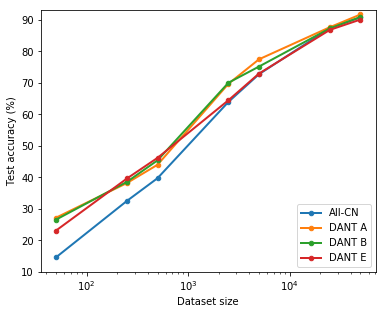
\includegraphics[width=0.31\linewidth]{chapter_7/figures/fig_1.png}
%		%\vspace{-2mm}
%		%\caption{AUC as a function of acquisition step}
%	\end{subfigure}
%	\hfill
%	\begin{subfigure}[]{}
%		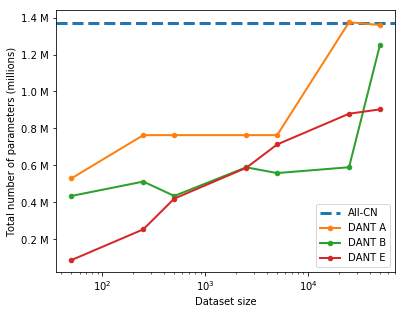
\includegraphics[width=0.32\linewidth]{chapter_7/figures/fig_2.png}
%		%\vspace{-2mm}
%		%\caption{\# of positive examples as a function of acquisition step}
%	\end{subfigure}
%	\hfill
%	\begin{subfigure}[]{}
%		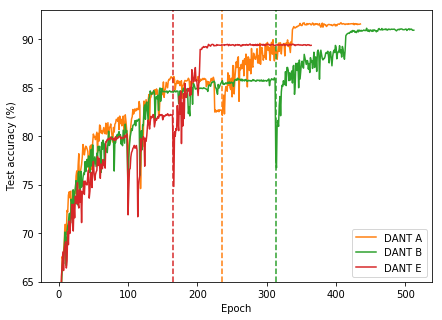
\includegraphics[width=0.33\linewidth]{chapter_7/figures/fig_3.png}
%		%\vspace{-2mm}
%		%\caption{\# of positive examples as a function of acquisition step}
%	\end{subfigure}
%	\vspace{-2mm}
%	\caption{Effect of varying datasize on the performance of discovered models.  }
%	\label{fig:adaptivemodel}
%\end{figure*}

%\begin{figure*}
%% https://tex.stackexchange.com/questions/56163/subfigure-error-missing-number-treated-as-zero
%\centering
%\subfigure[]{}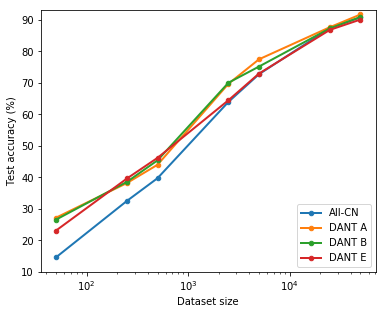
\includegraphics[width=0.4\linewidth]{chapter_7/figures/fig_1.png}
%\subfigure[]{}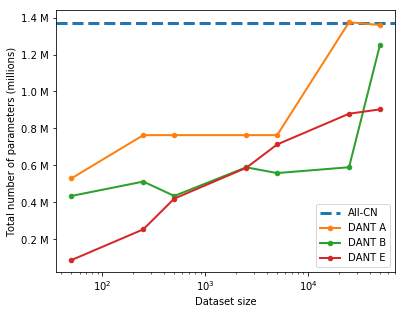
\includegraphics[width=0.4\linewidth]{chapter_7/figures/fig_2.png}
%\caption{Effect of varying datasize on the performance of discovered models.}
%
%\end{figure*}

%%%%%% (backup) Removed result section %%%%%%%%%%
%\subsection{Training time comparison (optional)}
%Tab.\ref{table:traintime} summarise the time taken on a single Titan X GPU for the growth phase and refinement phase of various ANTs, and compare against the training time of All-CN. The local optimisation during the growth phase means that the gradient computation is constrained to the newly added component of the graph, enabling to grow a good candidate model under $2$ hours on a single GPU. 
 
% attains up to $2.5$ times reduction in the required time in comparison with the synthetic experiment where each step of the growth phase is performed via global optimisation. 

 %%%%%% (backup) Removed result section %%%%%%%%%%
% \begin{table}
% 	%\vskip 0.1in  % Was 0.15in
% 	\begin{center}
% 		\begin{small}
% 			%\begin{sc}
% 			\begin{tabular}{l|c|c|c|c}
% 				\hline
% 				\multicolumn{1}{c}{} &  \multicolumn{2}{c}{\textbf{Growth}} & \multicolumn{2}{c}{\textbf{Fine-tune}}  \\
% 				\hline
% 				Model & Time & Epochs  & Time  & Epochs\\
% 				\hline
% %				\abovespace
% %				ANT-MNIST-1  &  &   &LC& 200 \\
% %				ANT-MNIST-2& &  & LC & 200\\
% %				ANT-MNIST-6 & &  &LC & 200 \\
% %				\hline
% 			%	\abovespace
% 				All-CN (baseline)&--~~~ & --~~~ & 1.1 (hr) &200 \\
% 				ANT-CIFAR10-A&1.3 (hr) & 236  & 1.5 (hr) &200 \\
% 				ANT-CIFAR10-B & 0.8 (hr) & 313 & 0.9 (hr) & 200\\
% 				ANT-CIFAR10-C&  0.7 (hr) &  285& 0.8 (hr) & 200 \\
% 				\hline
% 			\end{tabular}
% 			%	\end{sc}
% 		\end{small}
% 	\end{center}
% 	\vspace{-3mm}
% 	\caption{Training time comparison. Time and number of epochs taken for the growth and refinement phase are shown. along with the time required to train the baseline, All-CN.}
% 	\label{table:traintime}
% 	%\vskip 0.1in 
% \end{table}

%\subsection{Representational benefits of split}
%\textcolor{red}{No results yet!}. 
%It would be nice to demonstrate the benefits of splitting over going deeper. I am thinking of growing ANTs but only allowing them to go deeper. We can compare against the standard ANTs which also have the option to split. Hopefully, we get some nice results that quantitatively show the benefits of having an option to partition the data! 

%%%%%% (backup) Removed result section %%%%%%%%%%
%\subsection{Effect of training steps (optional)}
%Number of training steps at each stage in the growth phase affects the discovered architecture, and consequently the classification performance. If too few steps of optimisation are performed, then the added module (additional router or transformer) may simply not be tuned enough. On the other hand, if too many optimisation steps are taken, this causes the added component to overfit. Both extremes prevent the model from making a meaningful further growth. It is therefore important to find the right number of local training steps in order to perform an effective growth phase.

%Some preliminery experiments done. The main point I want to raise here is that underexploration or over-finetuning at local level is bad. You need to find the right amount of time spend at each step of the growth phase to maximize the power of our proposed algorithm. Automating this step is future work. 

% \subsection{EM and stochastic approximation}
% \textcolor{red}{No results yet!}. All the results reported so far are not based on EM. If we have time, it would be nice if we could show that EM performs better than standard back-propagation (not done yet). If not, then we may as well stick to the simpler optimisation algorithm. However, at least we should introduce the stochastic version, which is much lighter weight,  and show how much performance is sacrificed. This may be useful for the community as it may be the key to scale up the method. In the method section, we can briefly draw a connection between this stochastic method and EM, and discuss that one is just an approximation of the other. 

%\textbf{Local optima and weight resetting:} A snippet from S3.2 in \cite{real2017large}: 
%\textit{``the identity mutation offers a mechanism for populations to get trapped in local optima. Some individuals may get trained more than their peers just because they happen to have undergone more identity mutations. It may, therefore, occur that a poor architecture may become more accurate than potentially better architectures that still need more training. In the extreme case, the well-trained poor architecture may become a super-fit individual and take over the population.
%"}

\section{Discussion and Conclusion}
In this chapter, we introduced Adaptive Neural Trees (ANTs), a simple way to marry the architecture learning, conditional computation and hierarchical clustering of decision trees (DTs) with the hierarchical representation learning and gradient descent optimization of deep neural networks (DNNs). Our proposed training algorithm optimises both the parameters and architectures of ANTs through progressive growth, tuning them to the size and complexity of the training dataset. Together, these properties make ANTs a generalisation of previous work attempting to unite NNs and DTs. Finally, we validated the claimed benefits of ANTs for regression (SARCOS dataset) and classification (MNIST \& CIFAR10 datasets), whilst still achieving high performance. 

Future work will aim to scale up ANTs to medical imaging applications which typically involve larger, higher dimensional datasets. This requires training potentially wider and deeper ANTs, which necessitates a more effective and efficient optimisation algorithm. Firstly, the current growth procedure is greedy and suboptimal. The sub-optimality of the local decisions only gets worse as the tree gets more complex. In the future, we will look into different ways to alleviate this issue such as (1)  more global optimisation during growth phase, (2) merging of branches \cite{shotton2013decision} or (3) training in entangled settings as already done in decision tree research \cite{montillo2011entangled}. Secondly, for large trees, the global refinement phase would be computationally expensive since the associated computation involves every part of the tree structure. One potential solution to this is to employ a Monte-Carlo approximation of the training by stochastically traversing the tree, while using gradient estimators for learning the parameters of the routers such as REINFORCE and straight-through (ST) estimators \cite{bengio2013} or more modern methods such as Gumbel ST estimator \cite{jang2016categorical}, REBAR \cite{tucker2017rebar} and RELAX \cite{grathwohl2017backpropagation}. We have also limited ourselves to relatively simple NN components in the design of the ANT's primitive modules. As future work, we aim to extend ANTs to use more recent advances in deep learning, particularly residual learning \cite{he2016deep} and dense connections \cite{huang2017densely}, as these have enabled the successful optimisation of more performant NNs. 

%\textcolor{red}{Shouldn't we also mention that the architecture is not very stable at the moment. We can chalk this up to the optimisation. May be try to integrate this point in the above paragraph. }

Another important challenge is to explore the value of the learned hierarchical structures of ANTs  in terms of “interpretability” (or algorithmic transparency). I believe that the tree-shaped hierarchy provides a new means to understand its internal decision making process---for instance, given an image where the ANT fail to classify, you could compare against a large number of correctly predicted examples, and potentially localise a point of routing failure where the ANT makes the wrong decision. On the other hand, such localisation of failures is more difficult in conventional CNNs with a single fully distributed representation. In addition, such hierarchical and decomposed interpretations are complementary to existing visualisation techniques such as saliency based attribution methods \cite{guidotti2018survey}. For example, providing saliency maps of the series of routing decisions may potentially provide a layer of transparency into the decisions made in the raw feature space. 

% Currently, the predictive distributions from all existing paths on the tree are computed during training, which can become expensive for large models, especially during the fine-tuning phase based on global optimisation. To combat this issue, we experimented with various forms of MC approximations of the default training algorithm where each sample stochastically traverses the tree-structure, only engaging parameters on the selected root-to-leaf path.

% In contrast with the default soft routing decisions, however, the MC approximation operates on stochastic hard decisions i.e. samples from Bernouli random variables given by the routers, rendering backpropgation non-usable. We therefore used various gradient estimators, such as REINFORCE and straight-through (ST) estimator (Bengio, 2013, see option -r_sto and -no_r_soft) and Gumbel ST estimator (Eric et al., 2016, see option --router_gumbel). Although more efficient, we have observed aggravated quality of local optimisation, especially at deeper levels. REINFORCE is unbiased, but suffer from high variance while ST estimators are low-variance but biased. It may be worth trying in the future more advanced gradient estimators (unbiased and lower variance) such as RELAX.

%As future work, we aim to extend ANTs to use more recent advances in deep learning, particularly residual learning \cite{he2016deep} and dense connections \cite{huang2017densely}, as these have enabled the successful optimisation of more performant NNs. 

%Through a series of experiments on object classification datasets, we demonstrated that ANTs can achieve high accuracy while retaining most of the benefits of decision trees, such as hierarchical clustering and conditional computation. ANTs can also be applied to small datasets, as the training procedure performs model selection automatically.

%In the end, this paper makes steps towards answering the question of whether it is better to partition data, or learn yet another level of features. In introducing a new model and training algorithm, we limited ourselves to relatively simple NN components. However, recent work has shown the importance of skip-connections in optimising very deep neural networks \cite{he2016deep,huang2017densely}. In future work we plan to scale up and otherwise improve upon ANTs by exploring the use of residual \cite{he2016deep} and dense connections \cite{huang2017densely}, which we hope will allow us to bridge the performance gap between our current architectures and these state-of-the-art networks.

%\bibliography{bibliography}
%\bibliographystyle{icml2019}

%\newpage
% \twocolumn[
% \icmltitle{\Large Supplementary materials: Adaptive Neural Trees\\}
% ]
%\appendix
% 

% ------------------------ DO NOT DELETE --------------------------------
% %%% Table that shows the number of parameters for the ablation study %%%%%
% \section{Ablation study of different constituent modules}
% In this section, we investigate the roles of router and transformer modules on the performance of ANTs. 

% \begin{table}[h]
% 	\caption{Ablation study to compare the effects of different components of ANTs on the number of parameters\label{tab:ablationstudy_2}}
% 	\vspace{-2mm}
% 	\scriptsize
%     \center
% 	\begin{tabular}{|l|ccc|ccc|ccc|}
% 		\hline
% 		\multicolumn{1}{|c}{\textbf{Method}} &  \multicolumn{3}{|c|}{\textbf{Params. (Full)}} & \multicolumn{3}{|c|}{\textbf{Params. (Path)}} & \multicolumn{3}{c|}{\textbf{Params. (Path without routers)}}  \\
% 			& Default & No $\mathcal{R}$ & No $\mathcal{T}$ & Default & No $\mathcal{R}$ & No $\mathcal{T}$ & Default & No $\mathcal{R}$  & No $\mathcal{T}$ \\
% 		\hline
% 		ANT-MNIST-A & 101K & 82K & 74K & 85K & 82K & 22K & 49K & 82K & 8K\\
% 	    ANT-MNIST-B & 77K  & 54K & 57K & 51K & 54K & 15K & 44K & 54K & 8K\\
%         ANT-MNIST-C & 40K  & 3K  & 32K & 8K  &  3K &  9K & 6K  & 3K & 8K\\
% 		ANT-CIFAR10-A & 1.4M & 1.0M & 0.8M & 1.0M & 1.0M & 0.5M & 0.8M & 1.0M & 0.03M\\
%         ANT-CIFAR10-B & 0.9M & 0.6M & 0.4M & 0.6M & 0.6M & 0.2M & 0.4M & 0.6M & 0.03M\\
%         ANT-CIFAR10-C & 0.7M & 0.3M & 0.3M & 0.5M & 0.3M & 0.1M & 0.2M & 0.3M & $4\times 10^{-5}$M\\
% 		\hline
% % 		\hline
% % 		ANT-MNIST-A & 101K& 74K  & 82K  & 85K  &  22K    &  82K  & 49K  & 8K & 82K\\
% % 	    ANT-MNIST-B & 77K & 57K & 54K & 51K  & 15K &  54K   & 44K  & 8K & 54K\\
% %         ANT-MNIST-C & 40K & 32K &  3K& 8K   &  9K  &   3K  & 6K   & 8K & 3K\\
% % 		ANT-CIFAR10-A &1.4M & 0.8M   & 1.0M & 1.0M & 0.5M   & 1.0M & 0.8M & 0.03M &1.0M \\
% %         ANT-CIFAR10-B &0.9M & 0.4M  & 0.6M & 0.6M & 0.2M   & 0.6M & 0.4M  & 0.03M  & 0.6M\\
% %         ANT-CIFAR10-C &0.7M & 0.3M & 0.3M & 0.5M & 0.1M  & 0.3M & 0.2M  & $4\times 10^{-5}$M & 0.3M\\
% % 		\hline
% 	\end{tabular}
% 	\vspace{-2mm}
% \end{table}





\begin{figure*}[ht]
    \vspace{-4mm}
	\center
	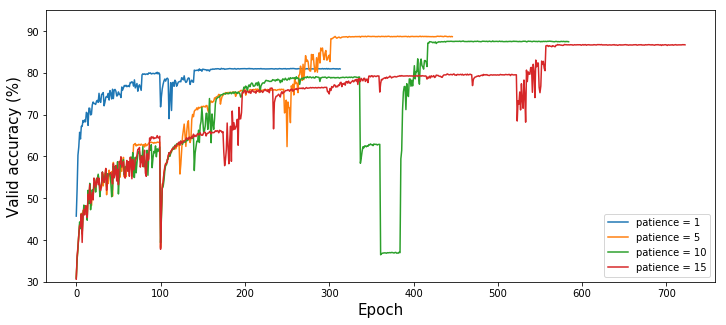
\includegraphics[width=0.7\linewidth]{figures/fig_patience.png}
    \vspace{-4mm}
	\caption{\small Effect of patience level on the validation accuracy trajectory during training. Each curve shows the validation accuracy on CIFAR-10 dataset.}
	\vspace{-4mm}
    \label{fig:patience}
\end{figure*}

\vspace{-2mm}
\section{Effect of training steps in the growth
\vspace{-2mm}
phase}\label{sec:supp_effect_of_patience}
Fig. \ref{fig:patience} compares the validation accuracies of the same ANT-CIFAR-C model trained on the CIFAR-10 dataset with varying levels of patience during early stopping in the growth phase. A higher patience level corresponds to more training epochs for optimising new modules in the growth phase. When the patience level is 1, the architecture growth terminates prematurely and plateaus at low accuracy at $80\%$. On the other hand, a patience level of 15 causes the model to overfit locally with  $87\%$. The patience level of 5 gives the best results with $91\%$ validation accuracy.

%A patience level of 1 leads the model to underfit with $80\%$ accuracy, while a patience level of 15 causes the model to overfit locally with  $87\%$ accuracy; in between these, the patience level of 5 gives the best results with a validation accuracy of $91\%$.}
%Figure. 1 shows that when too few steps of optimisation are performed e.g. patience level is 1, the architecture growth terminates prematurely and plateaus at low validation accuracy at 80\%, which is roughly 10\% lower than the best case with patience level of 5. On the other hand, if too many optimisation steps are taken e.g patience level 15, this causes the added component to overfit locally, and leads to nearly 4\% drop in accuracy. Tuning this hyperparameter of patience level is therefore integral to successful optimisations of ANTs.



\section{Expert specialisation}\label{sec:supp_expert_specialisation}
\vspace{-2mm}
We investigate if the learned routing strategy is meaningful by comparing the classification accuracy of our default path-wise inference against that of the predictions from the leaf node with the smallest reaching probability. Tab. \ref{tab:test_routers} shows that using the least likely ``expert" leads to a substantial drop in classification accuracy, down to close to that of random guess or even worse for large trees (ANT-MNIST-C and ANT-CIFAR10-C). This demonstrates that features in ANTs become specialised to the subsets of the partitioned input space at lower levels in the tree hierarchy. 

\begin{table}[h]
	\caption {Comparison of classification performance between the default single-path inference scheme and the prediction based on the least likely expert. \label{tab:test_routers}}
    \footnotesize
    \center
	\begin{tabular}{|l|c|c|}
		\hline
		\multicolumn{1}{|c}{\textbf{Module Spec.}} &  \multicolumn{1}{|c|}{\textbf{Error \%}} & \multicolumn{1}{c|}{\textbf{Error \%}}  \\
		&(Selected path) & (Least likely path)  \\
		\hline
		ANT-MNIST-A &0.69 & 86.18  \\
	    ANT-MNIST-B &0.73 & 81.98  \\
        ANT-MNIST-C &1.68 & 98.84  \\
		ANT-CIFAR10-A & 8.32 & 74.28  \\
        ANT-CIFAR10-B & 9.18 & 89.74  \\
        ANT-CIFAR10-C & 9.34 & 97.52  \\
		\hline
	\end{tabular}
\end{table}
\vspace{-4mm}
\section{Visualisation of discovered architectures}\label{sec:supp_architectures}
\vspace{-2mm}
Fig. \ref{fig:architectures} shows ANT architectures discovered on the MNIST (i-iii) and CIFAR-10 (iv-vi) datasets. We observe three notable trends. Firstly, a large proportion of the learned routers separate examples based on their classes (red histograms) with very high confidence (blue histograms). The ablation study in Sec.~5.~1 (Tab.~4 in the main text) shows that such hierarchical clustering benefits predictive performance, while the conditional computation enables more lightweight inference (Tab.~3 in the main text). Secondly, most architectures learn a few levels of features before resorting to primarily splits. However, over half of the architectures (ii-v) still learn further representations beyond the first split. Secondly, all architectures are unbalanced. This reflects the fact that some groups of samples may be easier to classify than others. This property is reflected by traditional DT algorithms, but not ``neural'' tree-structured models with pre-specified architectures \citep{laptev2014convolutional,frosst2017distilling,kontschieder2015deep,ioannou2016decision}. 
\begin{figure*}[ht]
	\center
	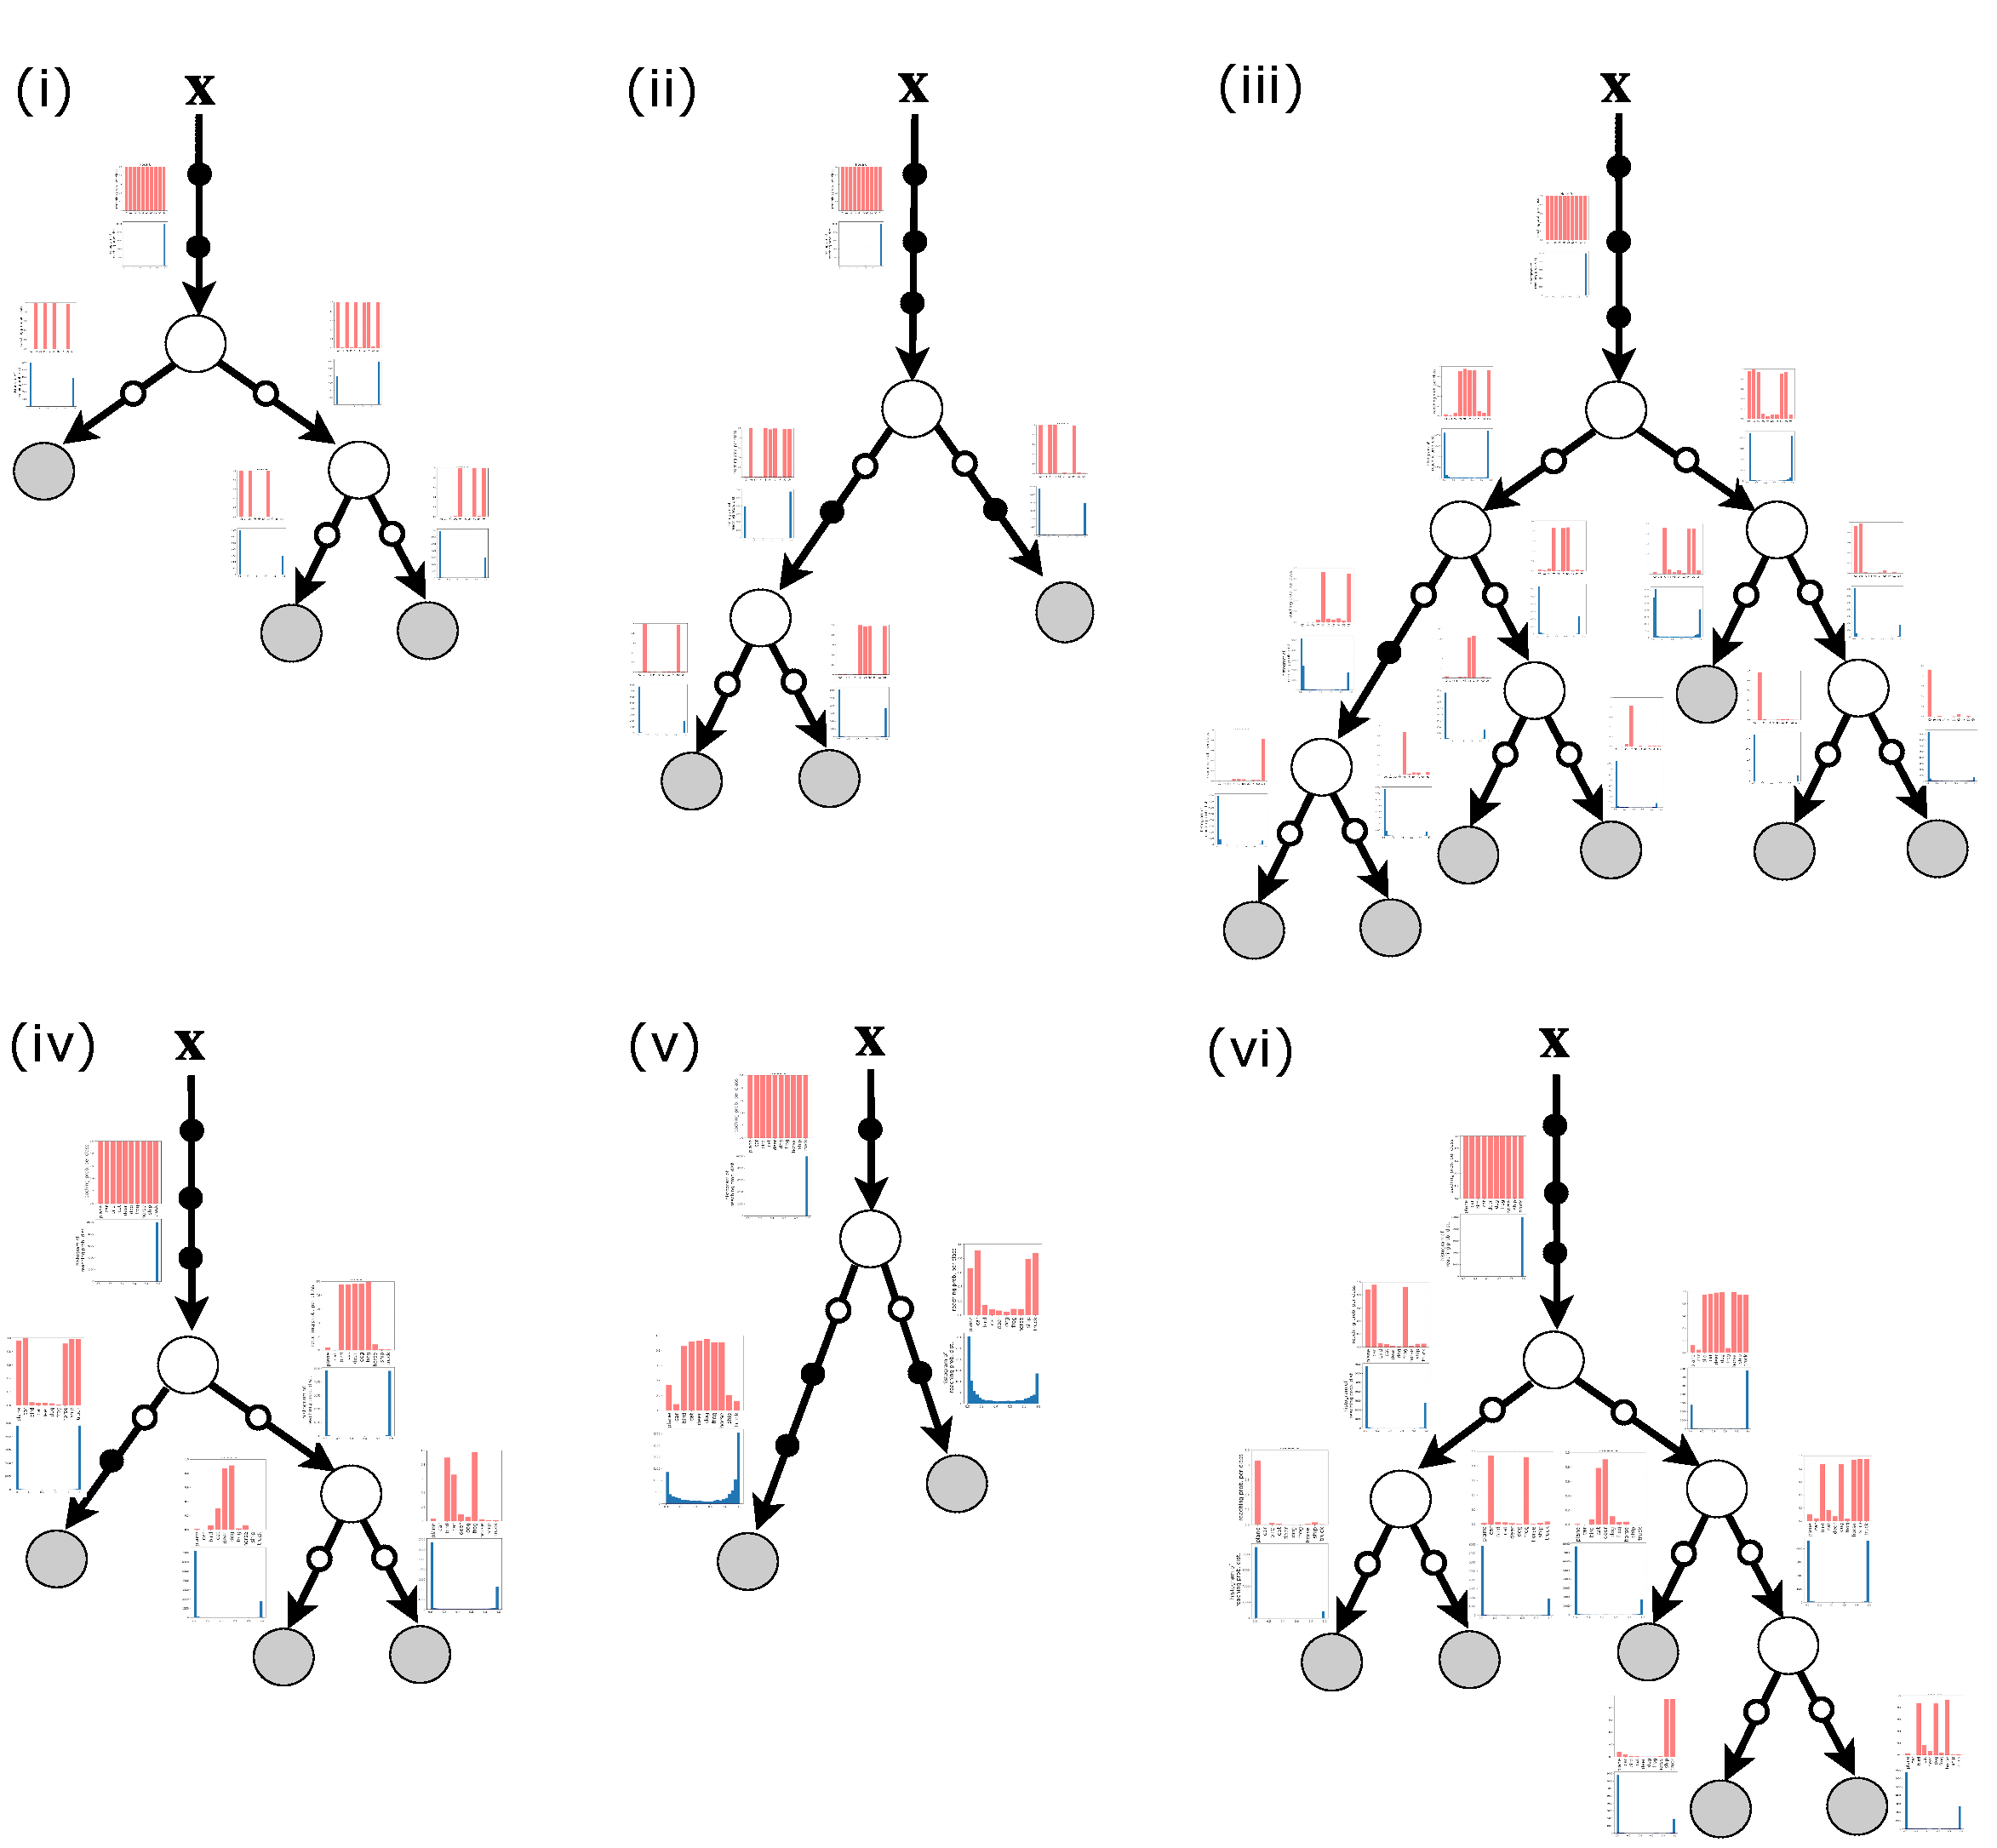
\includegraphics[width=0.8\linewidth]{figures/trees_all.pdf}
	\caption{\small Illustration of discovered ANT architectures. (i) ANT-MNIST-A, (ii) ANT-MNIST-B, (iii) ANT-MNIST-C, (iv) ANT-CIFAR10-A, (v) ANT-CIFAR10-B, (vi) ANT-CIFAR10-C. Histograms in red and blue show the class distributions and path probabilities at respective nodes. Small black circles on the edges represent transformers, circles in white at the internal nodes represent routers, and circles in gray are solvers. The small white circles on the edges denote specific cases where transformers are identity functions.}
	\label{fig:architectures}
\end{figure*}


% \section{Multivariate Regression}\label{sec:supp_regression}
% \vspace{-3mm}
% To demonstrate this, we also grow ANTs to perform (multivariate) regression on the SARCOS robot inverse dynamics dataset\footnote{\url{http://www.gaussianprocess.org/gpml/data/}}, which consists of 44,484 training and 4,449 testing examples, where the goal is to map from the 21-dimensional input space (7 joint positions, 7 joint velocities and 7 joint accelerations) to the corresponding 7 joint torques \citep{vijayakumar2000locally}. No dataset preprocessing or augmentation is used. We hold out 10\% of the training examples as a validation set. Baseline MLPs, routers and transformers are composed of single fully connected layers with 256 units with tanh nonlinearities, and the solver is a linear regressor. Other training details are the same as for classification (see Supp. Sec. \ref{sec:supp_train_details}). All non-NN-based methods were trained using scikit-learn \citep{pedregosa2011scikit}; only single-output GBT models were available so 7 separate GBTs were trained.

% The results are shown in Tab.~\ref{table:sarcos_results}. ANT-SARCOS outperforms all other methods in mean squared error with the full set of parameters, with GBTs performing slightly better using single-path inference. In comparison with results on MNIST and CIFAR-10, we note that the top 3 performing methods are all tree-based, with the third best method being an SDT (with MLP routers). This highlights the power of splitting the input space and conditional computation, both of which standard NNs are not capable of. Meanwhile, we still reap the benefits of representation learning, as shown by both ANT-SARCOS and the SDT (which is a specific form of ANT) requiring fewer parameters than the best-performing GBT configuration. Finally, we note that deeper NNs (5 vs. 3 hidden layers) can overfit on this small dataset, which makes the adaptive growth procedure of tree-based methods ideal for finding a model that exhibits good generalisation.

% \begin{table*}[ht]
% 	\caption{Comparison of performance of different models on SARCOS. The columns ``Error (Full)'' and ``Error (Path)'' indicate the mean squared error of predictions based on the full distribution and the single-path inference. The columns ``Params. (Full)'' and ``Params. (Path)'' respectively show the total number of parameters in the model and the average number of parameters utilised during single-path inference. ``Ensemble Size'' indicates the size of ensemble used to attain the reported accuracy. Results from \citet{zhao2017efficient} are included as a reference value from prior work, but are not directly comparable as they hold out 30\% of the training examples as a validation set.}
% 	\vspace{-3mm}
% 	\label{table:sarcos_results}
%     \center
%     \scriptsize
% 	\begin{tabular}{|c|l|cc|cc|c|}
% 		\hline
% 		& \multicolumn{1}{c|}{Method}
% 		& \multicolumn{1}{c}{\thead{\scriptsize Error \\ \scriptsize (Full)}}
% 		& \multicolumn{1}{c}{\thead{\scriptsize Error \\ \scriptsize (Path)}}
% 		& \multicolumn{1}{c}{\thead{\scriptsize Params. \\ \scriptsize (Full)}}
% 		& \multicolumn{1}{c|}{\thead{\scriptsize Params. \\ \scriptsize (Path)}}
% 		& \multicolumn{1}{c|}{\thead{\scriptsize Ensemble \\ \scriptsize Size}} \\	
% 		\hline
% 		\parbox[t]{2mm}{\multirow{11}{*}{\rotatebox[origin=c]{90}{SARCOS}}}
%         & Linear regression & 10.693 & N/A &\textbf{154}& N/A & 1 \\
%         & MLP with 2 hidden layers \citep{zhao2017efficient} & 5.111 & N/A & 31,804 & N/A & 1 \\
% 		& Decision tree & 3.708 & 3.708 & 319,591 & \textbf{25} & 1 \\
% 		& MLP with 1 hidden layer & 2.835 & N/A & 7,431 & N/A & 1 \\
%         & Gradient boosted trees & 2.661 & 2.661 & 391,324 & 2,083 & 7 $\times$ 30 \\
% 		& MLP with 5 hidden layers & 2.657 & N/A & 270,599 & N/A & 1 \\
% 		& Random forest & 2.426 & 2.426 & 40,436,840 & 4,791 & 200 \\
% 		& Random forest & 2.394 & 2.394 & 141,540,436 & 16,771 & 700 \\
% 		& MLP with 3 hidden layers & 2.129 & N/A & 139,015 & N/A & 1 \\
% 		&\cellcolor{gray!10}SDT (with MLP routers) &\cellcolor{gray!10} 2.118 &\cellcolor{gray!10} 2.246 &\cellcolor{gray!10} 28,045  &\cellcolor{gray!10} 10,167 &\cellcolor{gray!10} 1\\
% 		 & Gradient boosted trees & 1.444 & \textbf{1.444 }& 988,256 & 6,808 & 7 $\times$ 100 \\
% 		&\cellcolor{gray!10}ANT-SARCOS &\cellcolor{gray!10} \textbf{1.384} &\cellcolor{gray!10}  1.542 &\cellcolor{gray!10} 103,823  
% 		&\cellcolor{gray!10} 61,640 &\cellcolor{gray!10} 1\\
%       	\hline
% 	\end{tabular}
% \end{table*}

% \textbf{Ablation study:} we compare the regression error of our ANT in cases where the options for adding transformer or router modules are disabled (see Tab. \ref{tab:reg_ablationstudy}). In this experiment, patience levels are tuned separately for respective models. In the first case, the resulting models are equivalent to SDTs \citep{suarez1999globally} or HMEs \citep{jordan1994hierarchical} with locally grown architectures, while the second case is equivalent to standard NNs, grown adaptively layer by layer. We observe that either ablation consistently leads to higher regression errors across different module configurations. 
% \vspace{-3mm}
% \begin{table}[H]
% 	\caption{Ablation study to compare the effects of different components of ANTs on regression performance. ``NN'' refers to the case where the ANT is grown without routers while ``SDT/HME'' refers to the case where transformer modules on the edges are disabled. \label{tab:reg_ablationstudy}}
% 	\scriptsize
%     \center
% 	\begin{tabular}{|l|ccc|ccc|}
% 		\hline
% 		\multicolumn{1}{|c}{\textbf{Module Spec.}} &  \multicolumn{3}{|c|}{\textbf{Error (Full)}} & \multicolumn{3}{c|}{\textbf{ Error (Path)}} \\
% 			& ANT & NN & SDT/HME & ANT & NN & SDT/HME \\
% 			& (default) & (no routers) & (no transformers) & (default) & (no routers) & (no transformers) \\
% 		\hline
% 		ANT-SARCOS &1.384 & 2.511 & 2.118 &1.542 & 2.511 & 2.246 \\
% 		\hline
% 	\end{tabular}
% \end{table}
\vspace{-3mm}
\section{FLOPS}\label{sec:flops}
\vspace{-2mm}
Tab.\ref{tab:flops} reports the floating point operations per second (FLOPS) of ANT models for two inference schemes. The results for ResNet110 and DenseNet were retrieved from \cite{guan2017energy} and \cite{huang2018condensenet}, respectively. The FLOPs of all other models were computed using TorchStat toolbox available at \url{https://github.com/Swall0w/torchstat}. Using the single-inference reduces FLOPS in all ANT models to varying degrees.

\begin{table}[h]
% 	\caption {Comparison of classification performance between the default single-path inference scheme and the prediction based on the least likely expert. \label{tab:test_routers} between the }
    \caption{Comparison of FLOPs. \label{tab:flops}}
    \vspace{-5mm}
    \footnotesize
    \center
	\begin{tabular}{|c|l|c|c|}
		\hline
		&\multicolumn{1}{|c}{\textbf{Model}} &  \multicolumn{1}{|c|}{\textbf{FLOPS}} & \multicolumn{1}{c|}{\textbf{FLOPS}}  \\
		& &(multi-path) & (single-path)  \\
		\hline
		\parbox[t]{2mm}{\multirow{5}{*}{\rotatebox[origin=c]{90}{MNIST}}}
		&Linear Classifier & 8K & -   \\
		&LeNet-5 & 231 K & -  \\
		&ANT-MNIST-C & 99K & 83K  \\
	    &ANT-MNIST-B & 346K & 331K \\
        &ANT-MNIST-A & 382K & 380K  \\
        \hline
        
        \parbox[t]{2mm}{\multirow{7}{*}{\rotatebox[origin=c]{90}{CIFAR-10}}}&Net-in-Net & 222M &- \\
        &All-CNN & 245M & -\\
        &ResNet-110 & 256M&- \\
        &DenseNet-BC (k=24)& 9388M &- \\
		&ANT-CIFAR10-C & 66M & 61M  \\
        &ANT-CIFAR10-B & 163M & 149M  \\
        &ANT-CIFAR10-A & 254M & 243M  \\
		\hline
	\end{tabular}
\end{table}

\vspace{-5mm}
\section{Ensembling}\label{sec:supp_ensembling}
\vspace{-2mm}
As with traditional DTs \citep{breiman2001random} and NNs \citep{hansen1990neural}, ANTs can be ensembled to gain improved performance. In Tab.~\ref{tab:ensembling} we show the results of ensembling 8 ANTs (using the ``-A'' configurations for classification), each of which is trained with a randomly chosen split between training and validation sets. We compare against the single tree models, trained with the default split. In all cases both the multi-path and single-path inference performance is noticeably improved, and in MNIST we reach close to state-of-the-art performance (0.29\% versus 0.25\% \citep{sabour2017dynamic}) with significantly fewer parameters (851k versus 8.2M).
\vspace{-4mm}
\begin{table*}[ht]
	\caption{\small Comparison of prediction errors of a single ANT versus an ensemble of 8. \label{tab:ensembling}}
	\footnotesize
    \center
	\begin{tabular}{|l|cc|cc|cc|}
		\hline
		\multicolumn{1}{|c}{} &  \multicolumn{2}{|c|}{\textbf{MNIST} (Class Error \%)} &  \multicolumn{2}{|c|}{\textbf{CIFAR-10} (Class Error \%)} & \multicolumn{2}{c|}{\textbf{SARCOS} (MSE)}  \\
			& Multi-path & Single-path  & Multi-path & Single-path & Multi-path & Single-path   \\
		\hline
	    Single model & 0.64 & 0.69 & 8.31  & 8.32 & 1.384  & 1.542 \\	
        Ensemble & 0.29 & 0.30 & 7.76 & 7.79 & 1.226 & 1.372  \\
		\hline
	\end{tabular}
	\vspace{-4mm}
\end{table*}

\begin{table*}[ht]
	\caption{\small Parameter counts for a single ANT versus an ensemble of 8. \label{tab:ensembling_params}}
	\center
    \vspace{-1mm}
    \footnotesize
    \begin{tabular}{|l|cc|cc|cc|}
		\hline
		\multicolumn{1}{|c}{} &  \multicolumn{2}{|c|}{\textbf{MNIST} (No. Params.)} &  \multicolumn{2}{|c|}{\textbf{CIFAR-10} (No. Params.)} & \multicolumn{2}{c|}{\textbf{SARCOS}  (No. Params.)}  \\
			& Multi-path & Single-path  & Multi-path & Single-path & Multi-path & Single-path   \\
		\hline
	    Single model & 100,596 & 84,935 & 1.4M & 1.0M & 103,823 & 61,640 \\	
        Ensemble & 850,775 & 655,449 & 8.7M & 7.4M & 598,280 & 360,766  \\
		\hline
	\end{tabular}
	
	\vspace{-5mm}
\end{table*}

